%%%%%%%%%%%%%%%%%%%%%%%%%%%%%%%%%%%%%%%%%%%%%%%%%%%%%%%%%%%%%%%%%%%%%
%% This is a (brief) model paper using the achemso class
%% The document class accepts keyval options, which should include
%% the target journal and optionally the manuscript type. 
%%%%%%%%%%%%%%%%%%%%%%%%%%%%%%%%%%%%%%%%%%%%%%%%%%%%%%%%%%%%%%%%%%%%%

% Use single column for preprint.
\documentclass[journal=jpclcd,manuscript=letter]{achemso}
%\documentclass[journal=jpclcd,manuscript=letter,layout=twocolumn]{achemso}

%%%%%%%%%%%%%%%%%%%%%%%%%%%%%%%%%%%%%%%%%%%%%%%%%%%%%%%%%%%%%%%%%%%%%
%% Place any additional packages needed here.  Only include packages
%% which are essential, to avoid problems later. Do NOT use any
%% packages which require e-TeX (for example etoolbox): the e-TeX
%% extensions are not currently available on the ACS conversion
%% servers.
%%%%%%%%%%%%%%%%%%%%%%%%%%%%%%%%%%%%%%%%%%%%%%%%%%%%%%%%%%%%%%%%%%%%%
\usepackage{amsmath}
\usepackage{amssymb}
\usepackage{bbm}
\usepackage{booktabs}
\usepackage{placeins}
\usepackage{siunitx}
\usepackage{xcolor}
\usepackage{xr}

%%%%%%%%%%%%%%%%%%%%%%%%%%%%%%%%%%%%%%%%%%%%%%%%%%%%%%%%%%%%%%%%%%%%%
%% If issues arise when submitting your manuscript, you may want to
%% un-comment the next line.  This provides information on the
%% version of every file you have used.
%%%%%%%%%%%%%%%%%%%%%%%%%%%%%%%%%%%%%%%%%%%%%%%%%%%%%%%%%%%%%%%%%%%%%
%%\listfiles

%%%%%%%%%%%%%%%%%%%%%%%%%%%%%%%%%%%%%%%%%%%%%%%%%%%%%%%%%%%%%%%%%%%%%
%% Place any additional macros here.  Please use \newcommand* where
%% possible, and avoid layout-changing macros (which are not used
%% when typesetting).
%%%%%%%%%%%%%%%%%%%%%%%%%%%%%%%%%%%%%%%%%%%%%%%%%%%%%%%%%%%%%%%%%%%%%
\newcommand*\mycommand[1]{\texttt{\emph{#1}}}
\DeclareMathOperator{\Var}{Var}
\DeclareMathOperator{\tr}{tr}
\DeclareMathOperator{\Span}{span}
\DeclareMathOperator{\Div}{div}
\DeclareMathOperator{\Diag}{diag}
\DeclareMathOperator{\Id}{\mathbf{1}}
\DeclareMathOperator*{\argmin}{arg\,min}

% bold matrix
\newcommand\m[1]{\mathbf{#1}}
% bold vector
\renewcommand\vec[1]{\mathbf{#1}}

\setkeys{acs}{doi = true}
\SectionNumbersOn

% For referring to labels in the supporting information
\makeatletter
\newcommand*{\addFileDependency}[1]{% argument=file name and extension
  \typeout{(#1)}
  \@addtofilelist{#1}
  \IfFileExists{#1}{}{\typeout{No file #1.}}
}
\makeatother

\newcommand*{\myexternaldocument}[1]{%
    \externaldocument{#1}%
    \addFileDependency{#1.tex}%
    \addFileDependency{#1.aux}%
}
\myexternaldocument{supporting_information_long_version}


%%%%%%%%%%%%%%%%%%%%%%%%%%%%%%%%%%%%%%%%%%%%%%%%%%%%%%%%%%%%%%%%%%%%%
%% Meta-data block
%% ---------------
%% Each author should be given as a separate \author command.
%%
%% Corresponding authors should have an e-mail given after the author
%% name as an \email command. Phone and fax numbers can be given
%% using \phone and \fax, respectively; this information is optional.
%%
%% The affiliation of authors is given after the authors; each
%% \affiliation command applies to all preceding authors not already
%% assigned an affiliation.
%%
%% The affiliation takes an option argument for the short name.  This
%% will typically be something like "University of Somewhere".
%%
%% The \altaffiliation macro should be used for new address, etc.
%% On the other hand, \alsoaffiliation is used on a per author basis
%% when authors are associated with multiple institutions.
%%%%%%%%%%%%%%%%%%%%%%%%%%%%%%%%%%%%%%%%%%%%%%%%%%%%%%%%%%%%%%%%%%%%%
\author{Alexander Humeniuk}
\email{alexander.humeniuk@gmail.com}
\affiliation[]
{current address: Department of Chemistry, Graduate School of Science, Kyoto University, Kitashirakawa-Oiwakecho, Sakyo-Ku, Kyoto 606-8502, Japan}

%%%%%%%%%%%%%%%%%%%%%%%%%%%%%%%%%%%%%%%%%%%%%%%%%%%%%%%%%%%%%%%%%%%%%
%% The document title should be given as usual. Some journals require
%% a running title from the author: this should be supplied as an
%% optional argument to \title.
%%%%%%%%%%%%%%%%%%%%%%%%%%%%%%%%%%%%%%%%%%%%%%%%%%%%%%%%%%%%%%%%%%%%%
\title[]
  {Approximate Functionals for Multistate Density Functional Theory}
% Approximate functionals of the matrix density for density functional theory of ground and excited states

%%%%%%%%%%%%%%%%%%%%%%%%%%%%%%%%%%%%%%%%%%%%%%%%%%%%%%%%%%%%%%%%%%%%%
%% Some journals require a list of abbreviations or keywords to be
%% supplied. These should be set up here, and will be printed after
%% the title and author information, if needed.
%%%%%%%%%%%%%%%%%%%%%%%%%%%%%%%%%%%%%%%%%%%%%%%%%%%%%%%%%%%%%%%%%%%%%
\abbreviations{}
\keywords{excited states, time-independent density functional theory, multiconfigurational DFT, static correlation}

%%%%%%%%%%%%%%%%%%%%%%%%%%%%%%%%%%%%%%%%%%%%%%%%%%%%%%%%%%%%%%%%%%%%%
%% The manuscript does not need to include \maketitle, which is
%% executed automatically.
%%%%%%%%%%%%%%%%%%%%%%%%%%%%%%%%%%%%%%%%%%%%%%%%%%%%%%%%%%%%%%%%%%%%%
\begin{document}

%%%%%%%%%%%%%%%%%%%%%%%%%%%%%%%%%%%%%%%%%%%%%%%%%%%%%%%%%%%%%%%%%%%%%
%% The "tocentry" environment can be used to create an entry for the
%% graphical table of contents. It is given here as some journals
%% require that it is printed as part of the abstract page. It will
%% be automatically moved as appropriate.
%%%%%%%%%%%%%%%%%%%%%%%%%%%%%%%%%%%%%%%%%%%%%%%%%%%%%%%%%%%%%%%%%%%%%
\begin{tocentry}

%Some journals require a graphical entry for the Table of Contents.
%This should be laid out ``print ready'' so that the sizing of the
%text is correct.

%Inside the \texttt{tocentry} environment, the font used is Helvetica
%8\,pt, as required by \emph{Journal of the American Chemical
%Society}.

%The surrounding frame is 9\,cm by 3.5\,cm, which is the maximum
%permitted for  \emph{Journal of the American Chemical Society}
%graphical table of content entries. The box will not resize if the
%content is too big: instead it will overflow the edge of the box.

%This box and the associated title will always be printed on a
%separate page at the end of the document.

\end{tocentry}

%%%%%%%%%%%%%%%%%%%%%%%%%%%%%%%%%%%%%%%%%%%%%%%%%%%%%%%%%%%%%%%%%%%%%
%% The abstract environment will automatically gobble the contents
%% if an abstract is not used by the target journal.
%%%%%%%%%%%%%%%%%%%%%%%%%%%%%%%%%%%%%%%%%%%%%%%%%%%%%%%%%%%%%%%%%%%%%
\begin{abstract}
Recently Lu and Gao [J. Phys. Chem. Lett. 13, 33, 7762-7769 (2022)]
published a new, rigorous density functional theory for excited states and proved that the
projection of the kinetic and electron repulsion operators into the subspace of the lowest electronic states
are a universal functional of the matrix density $\m{D}(\vec{r})$.
This is the first attempt to find an approximation to the multistate universal functional $\m{\mathcal{F}}[\m{D}(\vec{r})]$.
It is shown that $\m{\mathcal{F}}$ (i) does not explicitly depend on the number of electronic states and (ii)
is an analytic matrix functional. 
The Thomas-Fermi-Dirac-von Weizs\"{a}cker model and the correlation energy of the homogeneous electron gas
are turned into matrix functionals guided by two principles: That each matrix functional should transform
properly under basis set transformations, and that the ground state functional should be recovered for a single electronic state.
Lieb-Oxford-like bounds on the average kinetic and electron repulsion energies in the subspace are given.
When evaluated on the numerically exact matrix density of LiF, this simple approximation
reproduces the matrix elements of the electron repulsion operator in the basis of the exact eigenstates accurately for all bond lengths.
In particular the off-diagonal elements of the effective Hamiltonian that come from the
interactions of different electronic states can be calculated with the same or better accuracy than the diagonal elements.
Unsurprisingly, the largest error comes from the kinetic energy functional.
More exact conditions that constrain the functional form of $\m{\mathcal{F}}$ are needed to go beyond the local density approximation.

% Diagonal and off-diagonal matrix elements of an effective Hamiltonian can be computed with matrix functional...
% Local density approximation Thomas-Fermi-Dirac-von Weizs\"{a}cker
% Lower bounds
% Recently Lu and Gao [J. Phys. Chem. Lett. 13, 33, 7762-7769 (2022)]
% published a new, rigorous density functional theory for excited states, in which the ground
% and excited states are treated on an equal footing. The fundamental variable is the projection
% of the one-particle density operator on the subspace of the lowest $N$ eigenstates.
% * Universal functional F does not depend on the number of states
% * F is an analytic matrix functional.
% This is the first attempt to find an approximation to the multistate universal functional.
%
% Two principles will guide the search for the multistate matrix functional:
% (a) The functional should transform properly under basis transformations.
% (b) For a single eletronic state, the functional form of an existing ground state functional should be recovered.
% These criteria are not enough to determine the functional uniquely. When in doubt, one of the simplest alternatives is chosen.
% How to incorporate 

% LDA-like functional
% test on LiH
% off-diagonal matrix elements of the effective Hamiltonian
\end{abstract}

%%%%%%%%%%%%%%%%%%%%%%%%%%%%%%%%%%%%%%%%%%%%%%%%%%%%%%%%%%%%%%%%%%%%%
%% Start the main part of the manuscript here.
%%%%%%%%%%%%%%%%%%%%%%%%%%%%%%%%%%%%%%%%%%%%%%%%%%%%%%%%%%%%%%%%%%%%%

% Suggested Reviewers:
%  - Dr. Yangyi Lu, Shenzhen Bay Laboratory China, luyy@szbl.ac.cn
%  - Prof. Jiali Gao, Chemistry Department, University of Minnesota, gao@jialigao.org
%  - Prof. Laura Gagliardi, University of Minnesota, gagliard@umn.edu
%  - Prof. Mark Casida, Université Grenoble Alpes, mark.casida@univ-grenoble-alpes.fr
%  - Prof. Andreas Görling, Universität Erlangen-Nürnberg, andreas.goerling@fau.de
%  - Prof. E. K. U. Gross, Max Planck Institute of Microstructure Physics Halle, hardy@mpi-halle.mpg.de
%  - Prof. Emmanuel Fromager, Laboratoire de Chimie Quantique, Institut de Chimie, CNRS/Université de Strasbourg, fromagere@unistra.fr
%  - Prof. Emily A. Carter, Princeton University, eac@princeton.edu
%  - author listed on "DFT exchange: sharing perspectives on the workhorse of quantum chemistry and materials science", 
%    Phys. Chem. Chem. Phys., 2022, 24, 28700, DOI: 10.1039/d2cp02827a
%

\section{Introduction}
%%%%% Motivation for developing multiconfigurational DFT
Kohn-Sham (KS) density functional theory (DFT) \cite{Hohenberg1964inhomogeneous,Kohn1965} is probably the single most used electronic structure
method in academia and industry, because it can be operated as a black box and often gives
reasonable answers without requiring excessive computational time.
For molecules, linear-response \cite{Casida1995} time-dependent \cite{Runge1984} DFT (LR-TDDFT) provides excited state properties very efficiently,
but it has problems with core-excitations \cite{Imamura2006time,Janesko2023projected},
doubly excited states \cite{Levine2006conical}, charge transfer states \cite{Dreuw2003long},
Rydberg states \cite{Dreuw2003long} and conical intersections to the ground state \cite{Levine2006conical}.
Although some of these issues can be fixed with tuned \cite{Stein2009reliable} range-separated \cite{Tawada2004long}
or projected \cite{Janesko2023projected} hybrid functionals or spin-flip DFT \cite{Shao2003spin},
whenever the electronic structure becomes more complicated, multi-reference wavefunction-based methods have to be employed.

In particular, (TD)-DFT fails when an excited state comes close in energy to the ground state,
which then cannot be described by a single Slater determinant. This happens at unstable molecular
geometries, when bonds are broken, such as in diradicals, at transition states and conical intersections.
% Near-degenerate spin states in transition metal coordination complexes are also problematic.
% Even the open-shell singlet state of the dissociated hydrogen molecule cannot  [I HAVE TO READ MORE ABOUT THIS]
In wavefunction theory (WFT) the near-degenerate states can be included in a multi-state treatment
through configuration interaction (CI) or multi-configurational self-consistent field (MC-SCF).
A few important configurations can capture the "static correlation" and give a qualitatively correct
electronic structure. The remaining configurations each have a very small weight in the wavefunction,
but since there are many of them, huge CI expansions are needed to get accurate, quantitative energies.
This energy contribution is termed the "dynamic correlation" energy.
The distinction between "static" and "dynamic" correlation is somewhat fuzzy, as it depends on the partitioning
of the Hilbert space into a few strongly interacting states and the rest. However, it is the treatment of the
"dynamic correlation" by perturbation theory or configuration interaction
that makes wavefunction-based methods so expensive. In density functional theory, on the other hand, the exchange-correlation
functional already accounts for the "dynamic correlation", while the "static correlation" is problematic.
Since DFT is formulated in terms of the electron density rather than wavefunctions, it is not clear how to compute
the interaction of states, which gives the off-diagonal elements in some effective Hamiltonian.
The central question in this article therefore is the following: 
How does one get the off-diagonal matrix elements for treating static correlation with DFT in a configuration-interaction-like manner?

%%%%% State of the art: Multi-configurational and variational DFT
The development of a multi-configurational and time-independent, variational DFT is an active research area,
but a far cry from the established TD-DFT.
A number of variational density-functional theories for excited states have been formulated, most notably
Theophilou's subspace DFT \cite{Theophilou1979}, Gross-Oliveira-Kohn ensemble DFT \cite{Gross1988ReyleighRitz} and
Levy \& Nagy's variational DFT for individual excited states \cite{Levy1999}.
In those theories, the universal excited-state functional depends on additional parameters apart from an electronic density,
which allow to distinguish between the excited state and the ground state: In ensemble density functional theory
\cite{Gross1988ReyleighRitz,Gross1988EnsembleDFT} there is a dependence on a vector of ensemble weights
and Levy \& Nagy's excited state functional \cite{Levy1999} depends on both the excited and the ground state densities.
In addition the functionals seem to depend on
the number of electronic states, so that a different functional would be needed for 2,3 etc. states:
In ensemble DFT the length of the weight vector changes with the number of states $N$;
in Levy and Nagy's theory the constrained search in Eqn.(2) of Ref.~\cite{Levy1999} is over all wavefunctions that are orthogonal
to the first $N-1$ states, which introduces an implicit dependence on $N$.
In G\"{o}rling's Kohn-Sham formalism for excited states the functionals
depends on the ground state density and the index of the excited state. \cite{Goerling1996density}
Ayers showed that the Coulomb interaction is special, because the density of an excited state of a Coulombic system also encodes
the excitation level, so that no additional parameters are needed. \cite{Ayers2012} The universal functional for
any electronic state depends only on the electronic density, provided that the external potential is Coulombic. \cite{Ayers2012}
However, although the existence of those universal functionals can be proven,
it is not clear how to approximate them for practical calculations
and if or how they differ from the ground state functional.

Deur et al. worked out the weight-dependent ensemble functional for the asymmetric Hubbard dimer \cite{Deur2017},
which is a two-state model for H$_2$. However, in the model, the "density" object is a vector of site occupations
and not on a real space density, therefore the findings are not transferable to realistic molecular Hamiltonians.

Most publications on time-independent DFT are formal. They derive their value from providing justification for
the use of some simpler theory such as $\Delta$SCF which employs a ground state functional.
Numerical calculations using variational DFT methods are rare and usually reuse the ground state functional.
Pastorczak at al. tested ensemble DFT methods on small molecules using ground state functionals or exact exchange
with self- and ghost-interaction corrections. \cite{Pastorczak2014} They found that the corrections
do not necessarily improve the energies and that ensemble DFT cannot compete with TD-DFT in terms of accuracy. \cite{Pastorczak2014}

% MSDFT
Multistate density functional theory (MSDFT)
\cite{Gao2016} predates the rigorous theorems of Lu and Gao \cite{Lu2022JPCL}
that establish a existence of a universal functional of the matrix density.
Originally MSDFT was developed as a hybrid between DFT and wavefunction theory (WFT) for treating multiconfigurational problems
that combines the best of both worlds. Dynamic correlation is incorporated
into the configurations by DFT, while static correlation is accounted for by letting the configurations interact.
Diagonalizing an effective Hamiltonian leads to the adiabatic eigenstates. MSDFT is akin to multiconfigurational wavefunction-based methods such
MCSCF or multireference configuration interaction (MRCI),
but has the advantage that only a minimal number of configurations is needed \cite{Lu2022fundamental} since DFT
is very good at handling the dynamic correlation. \cite{Leininger1997combining}

% MC-PDFT
Another approach for combining WFT and DFT is multiconfiguration pair-density functional theory (MC-PDFT). \cite{LiManni2014}
It uses CASSCF wavefunctions to calculate the kinetic energy, nuclear attraction and direct part of the electron-electron
repulsion energy, while the indirect part is computed from the one-particle density and the on-top pair density using
a new type of density functional. In this way double counting of the correlation energy is avoided.
Double counting can also be avoided by splitting the Coulomb interaction into a short- and a long-range part and
treating the first with DFT and the latter with WFT \cite{Leininger1997combining}.
A variational version of pair-density functional theory has been published recently. \cite{Scott2024}
Although the exact pair-density functional,
if it even exists, is unknown, ground state functionals of the total density and spin polarization can be "translated"
into functionals of the total density and on-top pair density. \cite{LiManni2014}
When states interact strongly around conical intersections or avoided crossings, they cannot be calculated separately as
this can lead to spurious crossings of potential energy surfaces. \cite{Sand2018state}
State-interaction pair-density functional theory (SI-PDFT)
\cite{Sand2018state} remedies this problem by diagonalizing the effective Hamiltonian in a final step.
The diagonal elements of the Hamiltonian come from 
MC-PDFT calculations for each state using the translated functional. 
For lack of a prescription for the off-diagonal Hamiltonian matrix elements in the DFT framework, a kind of diabatization
scheme is employed to get non-zero couplings between the states. \cite{Sand2018state}
A later multistate (MS) version of PDFT, called VMS-PDFT (V for variational), determines the unitary transformation
from the SA-CASSCF wavefunctions to a set of intermediate states, which give rise to off-diagonal couplings,
by maximizing the trace of the effective Hamiltonian. \cite{Bao2020multi} The dependence of the trace on the basis transformation
is an artifact of making different approximations to the diagonal and off-diagonal elements.
Sand et al. state that "the evaluation of off-diagonal elements in an effective Hamiltonian is not well-defined,
as no density functional that couples two interacting states is available". \cite{Sand2018state}
The purpose of this artice is to show
that it is indeed possible to obtain off-diagonal elements with the help of
matrix density functional theory, and that it is not necessary to treat diagonal and off-diagonal elements differently.
This observation might also be relevant for evaluating the diabatic couplings
of constrained DFT configuration interaction (CDFT-CI)\cite{Wu2007configuration}.
Depending on whether the adiabatic or some diabatic basis is chosen to represent the matrix density,
the matrix density functional will yield the corresponding adiabatic or diabatic Hamiltonian.
The trace of the effective Hamiltonian produced with a matrix functional is unitarily invariant by construction.

In general, existing variational DFT methods suffer from the lack of a clear route to designing new
functionals that go beyond repurposing existing KS-DFT functionals. The other open question is how
to compute matrix elements for state interactions consistently with density functional theory.

% Lu and Gao's rigorous MSDFT.
The rigorous, multistate DFT (MSDFT) theory by Lu and Gao \cite{Lu2022JPCL} might provide answers to those questions.
First of all, the universal functional only depends on a matrix representation of the one-particle density
operator, the \emph{matrix density}. The matrix density contains the densities of the electronic states on the diagonal
and the transition densities between them in the off-diagonal elements. It represents the electron density operator
in a subspace of electronic states. It should not be confused with the density matrix of a single electronic state.
Each matrix element is a function of space. And although the number of rows and columns of the matrix density is equal
to the number of electronic states that are considered, I will
argue that the functional of Lu and Gao does not depend on the number of states,
because it is an \emph{analytic matrix functional}.
This property suggests a simple path to an approximate multistate functional: by retaining the functional form
of an approximate ground state functional and replacing the scalar density with the matrix density \cite{lu_gao_2021_chemrxiv}.
The universal matrix functional provides not only the state energies but also the off-diagonal elements of the Hamiltonian.
Secondly, MSDFT resembles the state-averaged MCSCF of wavefunction theory,
however it is formulated in terms of electron densities and transition densities rather than wavefunctions.
The interaction between states is more transparent than in ensemble DFT,
where the densities of the individual states are combined into a single ensemble density,
whose physical meaning is not so obvious.

\textbf{Outline of the article:} Section \ref{sec:lu_gao_theorems} summarizes Lu and Gao's theorems and highlights
the importance of how the universal functional transforms under a change of basis.
Section \ref{ref:review_transition_functional} reviews the definitions of the
\emph{transition density functional} and the \emph{multistate correlation matrix functional}
and argues for partitioning the universal functional in such a way into Hartree, exchange and correlation
that each part transforms properly under basis transformations.
The basic recipe for translating ground state Kohn-Sham functionals into matrix density functionals by repurposing
the coefficients of their Taylor series and the limitations of this approach are outlined in section \ref{sec:basic_ideas_Taylor_series}.
This idea only works if the universal functional $\m{\mathcal{F}}[\m{D}(\vec{r})]$ has certain mathematical properties: 
Section \ref{sec:properties_analytic_matrix_functional} introduces the term \emph{analytic matrix functional} to characterize $\m{\mathcal{F}}$
and sketches a proof that $\m{\mathcal{F}}[\m{D}(\vec{r})]$ does not explicitly depend on the dimension of the subspace,
i.e. the dimension of the matrix $\m{D}(\vec{r})$.
In section \ref{sec:approximate_lda_msdft} a local density approximation to the universal functional is presented.
Section \ref{sec:exact_constraints} discusses incorporating exact conditions to constrain the multistate matrix functional.
Section \ref{sec:heg_msdft} explores whether there is a many-electron system for which the LDA multistate functional is exact.
Lieb-Oxford-style lower bounds on the average kinetic and electron repulsion energies in the subspace
are formulated in section \ref{sec:lower_bounds}.
The approximate functional is tested on the avoided crossing in LiF (section \ref{sec:results}).
%\label{sec:dicussion}
Section \ref{sec:conclusion} concludes.

\subsection{Rigorous MSDFT: Lu \& Gao's Theorems
\label{sec:lu_gao_theorems}
}
Recently Lu and Gao \cite{Lu2022JPCL} published a new, rigorous density functional theory for excited states, in which the ground
and excited states are treated on an equal footing. The fundamental variable is the projection
of the one-particle density operator $\hat{\rho}(\vec{r}) = \sum_{a=1}^{n} \delta(\hat{\vec{r}}_a - \vec{r})$ on the subspace
$\mathbb{V}^N$ of the lowest $N$ eigenstates, where $\hat{\vec{r}}_a$ is the position operator of electron $a$
and the sum goes over all $a=1,\ldots,n$ electrons.
The role of the scalar density $\rho(\vec{r})$
from the Hohenberg-Kohn theorem is taken by the multistate matrix density $\m{D}(\vec{r})$,
which is a matrix function of position $\vec{r}$
having the state densities $D_{II}(\vec{r}) = \rho_{I}(\vec{r})$ on its diagonal and the transition densities
$D_{IJ}(\vec{r}) = \langle \Psi_I \vert \sum_{a=1}^{n} \delta(\hat{\vec{r}}_a - \vec{r}) \vert \Psi_J \rangle$ on the off-diagonal.
Building on Theophilou's theorem \cite{Theophilou1979}, which states that the subspace of the lowest $N$ electronic states is uniquely
determined by the average density of those states, Lu and Gao prove two theorems that give access to the individual eigenenergies:

(1) Firstly they showed that the projection of the Hamiltonian operator onto the subspace $\mathbb{V}^N$ is a functional $\m{H}[\m{D}(\vec{r})]$ of the
matrix density $\m{D}(\vec{r})$. \cite[theorem 1]{Lu2022JPCL}
According to Theophilou's theorems \cite{Theophilou1979},
the subspace $\mathbb{V}^{N}$ is uniquely determined
by the average subspace density, $\rho_{\mathbb{V}^N}(\vec{r}) = \frac{1}{N} \sum_{I=1}^N D_{II}(\vec{r})$. Two matrix densities
$\m{D}(\vec{r})$ and $\m{D}'(\vec{r})$ having the same subspace density,
\begin{equation}
\frac{1}{N} \tr(\m{D}(\vec{r})) = \frac{1}{N} \tr(\m{D}'(\vec{r}))
\end{equation}
define the same subspace $\mathbb{V}^{N}$ and can only differ by a unitary transformation within the subspace. The
corresponding Hamiltonians $\m{H}'$ and $\m{H}$ differ by the same transformation. Therefore  $\m{D}(\vec{r})$
determines $\m{H}$ uniquely.
This multi-state analogue of the Hohenberg-Kohn theorem implies that the Hamiltonian can be split into an
external potential (the attractive nuclear potential which differs for each molecule) and a universal functional $\m{F}[\m{D}(\vec{r})]$ for the
electronic kinetic energy and electron-electron repulsion (that is the same for all systems):
\begin{equation}
 \m{H}[\m{D}(\vec{r})] = \m{\mathcal{F}}[\m{D}(\vec{r})] + \int d^3\!r ~ v(\vec{r}) \m{D}(\vec{r})
\end{equation}
Both $\m{H}$ and $\m{\mathcal{F}}[\m{D}(\vec{r})]$ are $N \times N$ matrices.

An important consequence of the fact that both $\m{D}(\vec{r})$ and $\m{H}[\m{D}(\vec{r})]$ are projections of operators onto the same subspace, is
that the universal matrix functional transforms bilinearly under a change of basis within the subspace. \cite[(3)]{Lu2022JPCL}
If the states in the subspace are transformed as $\vert \Psi_I' \rangle = \sum_{J=1}^N L^*_{IJ} \vert \Psi_J \rangle$,
the matrix density in the new basis becomes
\begin{equation}
D_{IJ}'(\vec{r}) = \langle \Psi_I' \vert \hat{\rho}(\vec{r}) \vert \Psi_J' \rangle
= \sum_{K,L=1}^{N} L_{IK} \langle \Psi_K \vert \hat{\rho}(\vec{r}) \vert \Psi_L \rangle L^*_{JL},
\end{equation}
or written in matrix notation
\begin{equation}
\m{D}'(\vec{r}) = \m{L} \m{D}(\vec{r}) \m{L}^{\dagger}.
\end{equation}
Similarly the Hamiltonian in the new basis becomes
\begin{equation}
\m{H}' = \m{L} \m{H} \m{L}^{\dagger}.
\end{equation}
This means that the universal functional has to transform as \cite{Lu2022JPCL}
\begin{equation}
 \m{\mathcal{F}}[\m{L} \m{D}(\vec{r}) \m{L}^{\dagger}] = \m{L} \m{\mathcal{F}}[\m{D}(\vec{r})] \m{L}^{\dagger} \label{eqn:F_basis_transformation}
\end{equation}
under a basis transformation $\m{L}$. Note that $\m{D}(\vec{r})$ is an $N \times N$ matrix function of $\vec{r}$,
but the basis transformation $\m{L}$ is just an $N \times N$ matrix.
 The relation \ref{eqn:F_basis_transformation} is very important, since it constrains
the search for matrix functionals to the class of \emph{analytic matrix functionals}, as will be explained later on.
It also implies that its functional form
is independent of the number of states in the subspace, so that the same functional holds for $N$ states or for a single state $1$.
An approximation to the universal matrix functional $\m{\mathcal{F}}[\m{D}(\vec{r})]$ automatically gives an approximate universal
functional of the ground state density $\mathcal{F}[\rho(\vec{r})]$. The reverse direction (deducing $\m{\mathcal{F}}[\m{D}(\vec{r})]$
from $\mathcal{F}[\rho(\vec{r})]$) is not so easy because of the non-commutativity of matrix multiplication.
Nevertheless relation \ref{eqn:F_basis_transformation} can guide the search for matrix functionals.

(2) Secondly Lu and Gao formulated a variational principle for finding the exact $\m{D}(\vec{r})$, which is a consequence of theorem 2
of Theophilou's subspace DFT. \cite{Theophilou1979}
Let the $N$ orthonormal trial vectors $\Psi_I'$ span the subspace $\mathbb{V}^{N'}$.
Then the average subspace energy, the multistate (MS) energy in the notation of Lu and Gao,
\begin{equation}
  E_{\text{MS}}[\{\Psi_I'\}] = \frac{1}{N} \sum_{I=1}^{N} \langle \Psi_I' \vert \hat{H} \vert \Psi_I' \rangle,
\end{equation}
of the trial space is larger or equal than
the subspace energy of the exact subspace (which is spanned by the exact lowest $N$ eigenstates $\Psi_I$),
\begin{equation}
E_{\text{MS}}[\mathbb{V}^N] \leq E_{\text{MS}}[\mathbb{V}^{N'}]
\end{equation}
Since according to Theophilou's theorems 3 to 5 the subspace is uniquely determined by the subspace density
$\rho_{\mathbb{V}^N}(\vec{r}) = \frac{1}{N} \sum_{I=1}^{N} D_{II}(\vec{r})$,
\begin{equation}
 \m{D}(\vec{r}) \longrightarrow \rho_{\mathbb{V}^N} \longrightarrow \mathbb{V}^N,
\end{equation}
it follows (theorem 2 of Lu and Gao \cite{Lu2022JPCL}) that the multistate energy of any trial matrix density $\m{D}'(\vec{r})$
is larger or equal to the exact multistate energy,
\begin{equation}
 E_{\text{MS}}[\m{D}(\vec{r})] \leq E_{\text{MS}}[\m{D}'(\vec{r})].
\end{equation}
The equality holds when the subspaces are the same $\mathbb{V}^N = \mathbb{V}^{N'}$, in which case $\m{D}'(\vec{r})$ and
the exact $\m{D}(\vec{r})$ as well as the Hamiltonians $\m{H}' = \m{H}[\m{D}'(\vec{r})]$ and the exact $\m{H}[\m{D}(\vec{r})]$, respectively,
 differ only by a basis transformation within the subspace. Therefore the subspace of the lowest eigenstates can be found by minimizing
$E_{\text{MS}}[\m{D}(\vec{r})]$ as a functional of $\m{D}(\vec{r})$.
Since the Hamiltonian in the basis of the eigenstates should be diagonal,
the eigenenergies can be obtained by diagonalizing the $N \times N$ matrix $\m{H}[\m{D}(\vec{r})]$.

(3) Lastly Lu and Gao proved that the matrix density can be represented exactly by no more than $N^2$ non-orthogonal, linearly-independent
Slater determinants built from $N^2$ different sets of $n$ molecular orbitals. \cite{Lu2022JPCL}
Optimizing the matrix density in terms of these auxiliary basis states ensures
that the matrix density is derived from antisymmetric wavefunctions. 
What kind of matrix function constitute a matrix density belonging to Fermionic wavefunctions is the
multistate version of the $N$-representability problem. Some obvious requirements are that the state densities should
integrated to the total number of electrons and that the transition densities should integrated to 0 to reflect that
eigenstates are orthonormal.
The question of parameterizing the matrix density will not be touched further.

The Hohenberg-Kohn (HK) theorem \cite{Hohenberg1964inhomogeneous} tells us that the ground state density $\rho_0(\vec{r})$
contains all information about the external potential $v(\vec{r})$
and as such it is formally possible to obtain the entire spectrum from the ground state density alone,
\begin{equation}
\rho_{0}(\vec{r}) \xrightarrow{\text{HK theorem}} v(\vec{r}) \longrightarrow \hat{H} = \hat{T} + \hat{W} + v(\vec{r}) \xrightarrow{\text{Schr\"{o}dinger eqn.}} \{ E_I, \Psi_I \}.
\label{eqn:HK_density_to_spectrum}
\end{equation}
However, this is of little practical use: Knowing that the mapping of Eqn.~\ref{eqn:HK_density_to_spectrum}
must exists provides no clue how to get from the left side to the right side.
 The matrix density $\m{D}(\vec{r})$ has the ground state density as its first element $\rho_{0}(\vec{r}) = D_{0,0}(\vec{r})$ on the diagonal
and therefore contains more information than strictly needed. For reference, in Theophilou's subspace DFT it is not possible to obtain the
ground state density $\rho_0(\vec{r})$ easily from the average subspace density $\rho_{\mathbb{V}^N}(\vec{r})$ without determining the subspace
$\mathbb{V}^N$, which is the difficult part.
%Of course the exact universal functional is unknown. 
The significance of the theorems by Lu and Gao, therefore, is not so much the existence of the mapping $\m{D}(\vec{r}) \to \m{H}$ (which is already
guaranteed by the HK theorem \cite{Goerling1996density}) but that their
universal matrix functional has the transformation property \ref{eqn:F_basis_transformation}.
This restricts the structure of the universal functional and gives some hints on how it can be approximated.

\subsection{Review of Approximate MSDFT Functionals
\label{ref:review_transition_functional}
}
Before embarking on the search for approximate matrix functionals,
the definition of the functional that should be approximated has to be clarified.
In MSDFT\cite{Gao2016} the diagonal elements
of the configuration interaction Hamiltonian $\m{H}$ are obtained by applying ground state Kohn-Sham (KS) theory to the state density $\rho_A$,
\cite[Eqn.~(3)]{Grofe2017} \cite[Eqn.~(12)]{Zhu2023}
\begin{equation}
 H_{AA} \approx E^{\text{KS}}[\rho_A]
\end{equation}
The coupling between the configurations is approximated by the matrix elements of the configurations (the WFT part)
and a \emph{transition density functional} (TDF), \cite[Eqn.~(5)]{Grofe2017}
\begin{equation}
 H_{AB} \approx \langle \Psi_A \vert \hat{H} \vert \Psi_B \rangle + \mathcal{E}^{\text{TDF}}_c[\rho_{AB}],
\end{equation}
$\langle \Psi_A \vert \hat{H} \vert \Psi_B \rangle$ captures the static and part of the dynamic correlation,
while the dynamic correlation that is still missing is added by the transition density functional.
$\mathcal{E}^{\text{TDF}}_c[\rho_{AB}]$ has been
approximated as the overlap-weighted average correlation energy of the interacting states, \cite[Eqn.~(6)]{Gao2016}
\begin{equation}
  \mathcal{E}^{\text{TDF}}_c[\rho_{AB}] = \frac{1}{2} S_{AB} \left( E_c^{\text{KS}}[\rho_A] + E_c^{\text{KS}}[\rho_B] \right),
\end{equation}
or by the multiplet-sum method \cite{Ziegler1977,Grofe2017} that allows to determine the coupling rigorously from the requirement that
states in a multiplet (same total spin $S$ but different spin projections $S_z$) are degenerate in the absence of a magnetic field.
These approximations make use of existing, Kohn-Sham density functional approximations (DFA)
for the ground state. These approximations are born out by encouraging benchmark calculations \cite{Zhu2023} on a varied set
of excitation energies in small molecules. However, in view of Lu and Gao's multistate equivalent of the Hohenberg-Kohn theorem,
which states that there is a one-to-one correspondence between the matrix density of the lowest few states and the Hamiltonian matrix,
it is clear that $\mathcal{E}^{\text{TDF}}_c$ cannot be a functional of a individual state densities $\rho_A$, $\rho_B$
or the transition density $\rho_{AB}$. Therefore Lu and Gao
replaced the transition density functional by a \emph{multistate correlation matrix functional} $\mathcal{E}_{c}[\m{D}]$, which depends
on the whole matrix density $\m{D}(\vec{r})$ rather than on the individual state or transition densities \cite{Lu2022fundamental}.

$\mathcal{E}_{c}[\m{D}(\vec{r})]$ is defined
as the difference between the universal functional $\mathcal{F}[\m{D}(\vec{r})]$ and an approximation $F_{\text{ms}}$ to it in the vector space spanned
by the auxiliary states $\{\Omega_A\}$
\cite[Eqn.~(30)]{Lu2022fundamental},
\begin{equation}
\mathcal{E}^{AB}_c[\{\Omega_A\}] = \mathcal{F}[\m{D}(\vec{r})]_{IJ}
- \underbrace{\langle \Omega_A \vert \hat{T} + \hat{W} \vert \Omega_B \rangle}_{F_{\text{ms}}[\{\Omega_A\}]}
\label{eqn:correlation_functional_auxiliary_basis_dependence}
\end{equation}
Note that the auxiliary basis functions that are sufficient to represent a matrix density $\m{D}(\vec{r})$ exactly, are not necessarily sufficient
to represent the exact many-electron wavefunctions of the subspace. In analogy to the Kohn-Sham determinant they are just a means to represent
the matrix density. In the way the correlation matrix is defined in Eqn.~\ref{eqn:correlation_functional_auxiliary_basis_dependence},
it depends on the auxiliary basis states that give rise to the matrix density $\m{D}(\vec{r})$. This is because the mapping from $\m{D}(\vec{r})$ back to
the wavefunctions is not unique, unless of course the auxiliary wavefunctions are equal to the lowest-energy eigenstates.
To turn $F_{\text{ms}}[\{\Omega_A\}]$
into a matrix functional $\mathcal{F}_{\text{ms}}[\m{D}(\vec{r})]$, which only depends on $\m{D}(\vec{r})$, Lu and Gao \cite{Lu2022fundamental} perform a
constrained minimization over the (orthogonal) auxiliary states to find the subset that minimizes the expectation value of $F_{\text{ms}}$
\cite[Eqn.~(28)]{Lu2022fundamental}, while keeping the matrix density $\m{D}(\vec{r})$ constant,
\begin{equation}
  \{\Omega_A^{\text{min}}\} = \argmin_{\{\Omega_A\}} \left\{ \sum_{I=1}^{N} 
    \langle \Omega_I \vert \hat{T} + \hat{W} \vert \Omega_I \rangle \quad \Big\vert \quad \{\Omega_A\} \to \m{D}(\vec{r}) \right\}
    \label{eqn:constrained_search}
\end{equation}
Then 
\begin{equation}
\mathcal{F}_{\text{ms}}[\m{D}(\vec{r})]_{AB} = \langle \Omega_A^{\text{min}} \vert \hat{T} + \hat{W} \vert \Omega_B^{\text{min}} \rangle
\end{equation}
is truely a functional of $\m{D}(\vec{r})$ and the correlation matrix can be defined as
\begin{equation}
 \mathcal{E}_{c}[\m{D}(\vec{r})] = \mathcal{F}[\m{D}(\vec{r})] - \mathcal{F}_{\text{ms}}[\m{D}(\vec{r})].
 \label{eqn:correlation_functional_matrix_functional}
\end{equation}
This functional is not readily computable, since the constrained search while keeping the density fixed cannot be performed.
In practice the multistate energy is minimized by changing the molecular orbitals and configuration coefficient of the auxiliary
wavefunctions, which then determine the matrix density. During the MCSCF-like minimization,
the auxiliary wavefunctions are not necessarily the minimum of the constrained
search of Eqn.~\ref{eqn:constrained_search}. The definition in Eqn.~\ref{eqn:correlation_functional_matrix_functional}
is rigorous but purely formal. For actual calculations it would be necessary to find approximations for the correlation matrix
as defined in Eqn.~\ref{eqn:correlation_functional_auxiliary_basis_dependence}, which is not a well-defined problem.

For a single electronic state, $\{\Omega_A^{\text{min}}\}$ turns into the Hartree-Fock determinant $\Psi_{\text{HF}}$ and $\mathcal{E}_c$
becomes the correlation energy. This is the quantum chemist's definition of the correlation energy as the energy that is missed by
Hartree-Fock theory. \cite[2.2.7]{Szabo_Ostlund_book}
In Hartree-Fock theory the correlation energy is measured relative to the minimum of the
expectation value of a single Slater determinant, while in MSDFT it is defined relative
to the minimum in a partially interacting active space. \cite{Lu2022JPCL}
On the other hand, in Kohn-Sham DFT exchange and correlation
are often approximated together. The exchange-correlation energy is defined as the difference between the total electron-repulsion
and the direct (classical) part of the Coulomb interaction. \cite{Lieb1979}
This has the advantage that it allows a definition of the exchange-correlation energy in terms of the density alone
without reference to any non- or partially-interacting wavefunctions.

It seems difficult to find good approximations to $\m{\mathcal{E}}_c[\m{D}(\vec{r})]$ as defined in Eqn.~\ref{eqn:correlation_functional_matrix_functional},
since the functional would need to know how much dynamic correlation is already included via
the auxiliary wavefunctions. LDA, GGA or even hybrid functionals designed for the ground state are probably too simple for that task.
Although theorem 3 of Lu and Gao \cite{Lu2022JPCL} guarantees that there is a minimal number of non-orthogonal \cite{Lu2022JPCL}
or orthogonal \cite{Lu2022fundamental} auxiliary basis functions, one could also use a larger space of auxiliary wavefunctions to
represent $\m{D}(\vec{r})$. But this affects the defintion of $\mathcal{E}_{c}$. In particular, if the auxiliary basis functions are
allowed to include the exact eigenfunctions of the Hamiltonian, the correlation energy $\m{\mathcal{E}}_c$ would be zero, since in this case
$\m{\mathcal{F}} = \m{\mathcal{F}}_{\text{ms}}$.

% In this article I try to find ...
This article tries to find approximations to the entire universal functional $\m{\mathcal{F}}[\m{D}(\vec{r})]$
(not just the residual correlation $\m{\mathcal{E}}_c$), even though this involves an approximate
matrix functional for the kinetic energy $\m{T}[\m{D}(\vec{r})]$, which comes with a very large error.
The exchange-correlation matrix functional
is defined as the difference between the matrix of the electron-repulsion operator in the subspace of the exact, lowest eigenstates
$\{\Psi_{I}^{\text{exact}}\}$ and
the multistate Hartree functional $\m{J}[\m{D}(\vec{r})]$,
\begin{equation}
 \text{XC}[\m{D}(\vec{r})]_{IJ} = \langle \Psi_I^{\text{exact}} \vert \sum_{a < b} 1/r_{ab} \vert \Psi_J^{\text{exact}} \rangle - J[\m{D}(\vec{r})]_{IJ}.
\end{equation}
$J[\m{D}(\vec{r})]$ contains the Coulomb interactions between state densities
and between state densities and transition densities both in the diagonal and the off-diagonal terms. It transforms 
in the same manner like $\mathcal{F}[\m{D}(\vec{r})]$, just as a proper matrix functional should.
This partitioning of the energy is independent of the choice of the auxiliary basis functions.
For a single electronic state the multistate Hartree functional $\m{J}[\m{D}(\vec{r})]$ reduces to the classical Coulomb interaction
$\frac{1}{2} \int \int' \frac{\rho(\vec{r}) \rho(\vec{r}')}{\vert \vec{r} - \vec{r}' \vert}$ and the multistate exchange-correlation matrix $\m{\text{XC}}[\m{D}]$
turns into the ground state exchange-correlation energy $E_{xc}[\rho]$ (without the kinetic contribution of Kohn-Sham theory),
even if the exact eigenstates are used to parameterize the matrix density.
This allows to reuse a ground state functional $E_{xc}[\rho]$ for $\text{XC}[\m{D}(\vec{r})]$, although the conversion of
a scalar functional into a matrix functional is not without ambiguities, because matrix multiplication is not commutative.

% Partitioning of universal functional in Hartree, exchange and correlation.
Some subtle differences between the notation in Lu et al. \cite{Lu2022JPCL,Lu2022JCTC} and this work are worth pointing out:
The electron repulsion energy is partitioned slightly differently into a Hartree, exchange and correlation part.
In analogy with the Kohn-Sham scheme \cite{Kohn1965}, Lu et al. compute the kinetic energy from the auxiliary Slater determinants (basis states).
They call the matrix elements of the electron-repulsion between the basis states,
$\langle \Phi_A \vert \hat{W} \vert \Phi_B \rangle$, the "Hartree and exchange-interaction matrix".
In this way some static and dynamic correlation is included in the Hartree and exchange part.
The difference with the exact universal functional is lumped in the the correlation functional, which takes the
form $\mathcal{E}_c = \mathcal{F}[\m{D}] - (\m{T}_{ms} + \m{E}_{Hx})$ \cite[Eqn.~(22)]{Lu2022JPCL}
and contains some kinetic contribution.
Evaluating the kinetic energy from orbitals
makes perfectly sense, since as of now there are no reliable orbital-free kinetic energy functionals, anyway.
Using a ground state functional for $\mathcal{E}_c$ can lead to doubly counting of correlation,
although the negligible energy difference between between ground state energies computed with MSDFT and KS-DFT
suggests that there is little double counting. \cite{Zhu2023} However, because all the complexity is packed into one
functional, it is difficult to reason about the properties of $\mathcal{E}_c$.

I define the kinetic energy $\m{T}[\m{D}]$, Hartree $\m{J}[\m{D}]$, exchange $-\m{K}[\m{D}]$ and correlation energy
$\m{C}[\m{D}]$ such that each is a functional of the matrix density and behaves properly under basis transformations
of the state vectors.
Auxiliary basis states are not used to compute any parts of the Hamiltonian.

\subsection{Basic Idea of Translating KS Functionals for MSDFT
\label{sec:basic_ideas_Taylor_series}
}
An important open question is how to find approximate multistate density functionals. 
In a preprint on Chemrxiv \cite{lu_gao_2021_chemrxiv} Lu and Gao mention that a local ground state functional
can be turned into a matrix functional by applying it to the eigenvalues of the matrix density.
I wish to investigate this idea further.

In the local density approximation (LDA) the exchange-correlation and kinetic energy \emph{functionals} of the density $\rho(\vec{r})$,
$E_{xc}[\rho]$ and $T[\rho]$, respectively,
are approximated by integrals over \emph{functions},
\begin{align}
  E_{xc}[\rho(\vec{r})] &= \int d^3\!r ~ \epsilon_{xc}(\rho(\vec{r})), \\
  T[\rho(\vec{r})] &= \int d^3\! ~ t(\rho(\vec{r})).
\end{align}
% The definition of $\epsilon_{xc}$ differs from the usual one, it is not the xc-energy per particle, so there is no additional factor of
% $\rho$ under the integral.
The energy density $\epsilon_{xc}(\rho)$ and the kinetic energy density $t(\rho)$ are functions
of a scalar variable. Let us call such a function $f: \mathbb{R} \mapsto \mathbb{R}$.
Assuming that $f$ is an analytic function, so that all the derivatives $f^{(k)}(\rho) = \frac{d^k f}{d\rho^k}$ exist,
$f$ can be expanded in a Taylor series around $\rho=0$,
\begin{equation}
 f(\rho) = \sum_{k=0}^{\infty} \frac{1}{k!} f^{(k)}(0) \rho^k.
\end{equation}
Now it is easy to turn the function $f(\rho)$ into a matrix function $\m{f}(\m{D}) : \mathbb{R}^{N \times N} \mapsto \mathbb{R}^{N \times N}$
of the matrix density $\m{D}$, by taking the coefficient of the Taylor series and replacing $\rho$ by $\m{D}$,
\begin{equation}
 \m{f}(\m{D}) = \sum_{k=0}^{\infty} \frac{1}{k!} f^{(k)}(0) \m{D}^k,
\end{equation}
where $\m{D}^k = \underbrace{\m{D} \cdot \m{D} \cdot \ldots \cdot \m{D}}_{\text{$k$ times}}$ is the $k$-th matrix power.
The corresponding LDA matrix functional $\m{F}[\m{D}]$ becomes
\begin{equation}
 \m{F}[\m{D}(\vec{r})] = \int d^3\!r ~ \m{f}(\m{D}(\vec{r})).
\end{equation}
A matrix function can simply be computed by applying the scalar function to each of its eigenvalues, but the definition
via the Taylor series generalizes more easily to the multivariate case.

If the scalar functional $F[\rho]$ only depends on the total electronic densities (summed over spins), as in the LDA,
this procedure determines a unique matrix functional $\m{F}[\m{D}]$.
However, to account for inhomogeneity or spin-polarization,
the energy density function has to depend on multiple arguments. For example, the exchange-correlation energy density in
the generalized gradient approximation (GGA), $\epsilon_{xc}(\rho(\vec{r}),\nabla \rho(\vec{r}))$, 
or the von-Weizs\"{a}cker kinetic energy density $t_{\text{vW}}(\rho(\vec{r}),\nabla \rho(\vec{r}))$ are functions of both the density and its gradient.
To translate a function $f(\rho,\nabla \rho)$ into a matrix function $\m{f}(\m{D},\nabla \m{D})$,
we follow the same recipe as for the single variable case, and expand $f$ into a multivariate Taylor series.
Denoting the partial derivatives by $f^{(m,n)} = \frac{\partial^{m+n} f}{\partial \rho^{m} (\nabla \rho)^{n}}(0,0)$, the first few terms
of the series around $(\rho,\nabla \rho) = (0,0)$ are,
\begin{equation}
 f(\rho,\nabla \rho) = f(0,0) + f^{(1,0)}~\rho + f^{(0,1)} ~ \nabla \rho + \frac{1}{2} f^{(1,1)} ~ \rho(\nabla \rho) + \ldots.
\end{equation}
When substituting the matrices $\m{D}$,$\nabla \m{D}$ for the scalar variables $\rho,\nabla \rho$, ambiguities arise,
because in matrix multiplication the order of the factors matters. It is not clear, for instance,
if the term $\rho (\nabla \rho)$
should be replaced by $\m{D} \cdot \nabla  \m{D}$ or by $\nabla \m{D} \cdot \m{D}$
or the average of the two. Since $\m{D}(\vec{r})$ and $\nabla \m{D}(\vec{r})$ do not commute,
$[\m{D}(\vec{r}),\nabla \m{D}(\vec{r})] \neq 0$, any order of factors will give
a different matrix functional.

Similar ambiguities arise with the local spin-density approximation (LSDA),
where $\epsilon_{xc}(\rho^{\uparrow}(\vec{r}), \rho^{\downarrow}(\vec{r}))$
depends on the spin-up and spin-down densities, since the matrix densities for different electron spins
in general do not commute, $[\m{D}^{\uparrow}(\vec{r}), \m{D}^{\downarrow}(\vec{r})] \neq 0$.

One sees that from one multivariate ground state functional an infinite number of matrix-density functionals can be derived.
The indeterminacy can be reduced to some extent by enforcing known properties of the exact multistate functional.
For example, the multistate-equivalent of the von-Weizs\"{a}cker kinetic energy functional should yield the
exact kinetic energy matrix for one-electron systems.

\section{Theory}
In the following the subscripts $a,b = 1,\ldots,n$ enumerate electrons, Latin captial letters $A,B,C,D,I,J,K,L,Y,Z = 1,\ldots,N$
enumerate electronic states in the subspace and $\alpha,\beta=x,y,z$ are Cartesian components of a three-dimensional vector.
Superscripts $^\alpha$,$^\beta$ denote the electronic spin. Atomic units are used throughout.

\subsection{Properties of the Matrix Density Functional.
\label{sec:properties_analytic_matrix_functional}
}

% Start with a gentle introduction:
%  1) What is a function? f(x): x --> f(x)
%  2) What is a functional? f[x(t)] --> for instance f[x] = \int x(t) dt
%  3) What is a matrix function? M(x)
%  4) What is an analytic function? --> admits a Taylor expansion
%  5) Now define the analytic matrix functional

\textbf{$\mathcal{F}[\m{D}(r)]$ is an analytic matrix functional.}
Since $\m{D}(\vec{r})$ is the projection of $\hat{\rho}(\vec{r})$ into the subspace $\mathbb{V}^{N}$, while ${\mathcal{H}[\m{D}(\vec{r})] = \mathcal{F}[\m{D}(\vec{r})] + \int d^3r ~ v(\vec{r}) \m{D}(\vec{r})}$ is the projection of the Hamiltonian $\hat{H}$, the matrix density functional has to transform under an arbitrary basis transformation $\m{L} : \mathbb{C}^{N \times N} \to \mathbb{C}^{N \times N}$ as \cite{Lu2022JPCL}
\begin{equation}
\mathcal{F}[\m{L} \m{D}(\vec{r}) \m{L}^{-1}] = \m{L} \mathcal{F}[\mathbf{D}(\vec{r})] \mathbf{L}^{-1} \label{eqn:basis_transformation_symmetry}
\end{equation}
This transformation property implies that $\mathcal{F}$ is an \emph{analytic matrix functional}. As we know, an analytic function of a scalar variable, $f(z): \mathbb{C} \to \mathbb{C}$ is defined by its Taylor series around some point $z_0$:
\begin{equation}
f(z) = \sum_{k=0}^{\infty} \frac{f^{(k)}}{k!} (z-z_0)^k
\end{equation}
With the help of the Taylor series the scalar function can be turned into a analytic matrix function, $f(\m{Z}): \mathbb{C}^{N \times N} \to \mathbb{C}^{N \times N}$, where the product of complex numbers is replaced by the matrix product
\begin{equation}
f(\m{Z}) = \sum_{k=0}^{\infty} \frac{f^{(k)}}{k!} (\m{Z} - z_0 \m{I})^k
\end{equation}
where $\m{I}$ is the identity matrix. If the Taylor series converges everywhere, we can expand around $z_0 = 0$ without loss of generality.
The coefficients $f^{(k)}$ are independent of the matrix dimension. Under a similarity transformation, an analytic matrix function behaves as
\begin{equation}
\begin{split}
  f(\m{L} \m{Z} \m{L}^{-1}) &= \sum_{k=0}^{\infty} \frac{f^{(k)}}{k!} (\m{L} \m{Z} \m{L}^{-1})^k \\
  &= f^{(0)} \underbrace{\m{L} \m{L}^{-1}}_{\m{I}} \m{I}
  + f^{(1)} \m{L} \m{Z} \m{L}^{-1}
  + \frac{f^{(2)}}{2} \m{L} \m{Z} \underbrace{\m{L}^{-1} \m{L}}_{\m{I}} \m{Z} \m{L}^{-1}
  + \ldots
  + \frac{f^{(k)}}{k!} \m{L} \m{Z}^k \m{L}^{-1} + \ldots \\
  &= \m{L} f(\m{Z}) \m{L}^{-1}.
\end{split}
\end{equation}
The definitions of analytic matrix functions in terms of a Taylor series or the transformation property are equivalent. \cite{Rinehart1955} 
An analytic matrix \emph{functional} $\mathcal{F}[\m{D}(\vec{r})] : (L^1)^{N \times N} \to \mathbb{C}^{N \times N}$ takes a matrix of $L^1$-integrable functions, which depend on the 3-dimensional spatial coordinate vector $\vec{r}$, as an argument.
If we interpret $\mathcal{F}$ as a general functional of $N^2$ functions, its functional Taylor expansion around $\m{D}(r) = 0$ would be
\begin{equation}
  \begin{split}
    \mathcal{F}[\m{D}(\vec{r})] & = \sum_{k=0}^{\infty} \frac{1}{k!} \int d^3\!r_1 d^3\!r_2 \cdots d^3\!r_k ~ \\
    & \quad \sum_{A,B,C,D,\ldots}^{N} \frac{\delta^{k} \mathcal{F}[\m{D}(\vec{r})]}{\delta D_{AB}(\vec{r}_1) \delta D_{CD}(\vec{r}_2) \ldots \delta D_{YZ}(\vec{r}_k)} D_{AB}(\vec{r}_1) D_{CD}(\vec{r}_2) \ldots D_{YZ}(\vec{r}_k).
  \end{split}
\end{equation}
where the Taylor coefficients are themselves $N^{2 k}$-dimensional tensors of functionals of the spatial coordinates $\vec{r}_1,\ldots,\vec{r}_k$.
However, because of the transformation property of Eqn.~\ref{eqn:basis_transformation_symmetry} the Taylor expansion of the matrix density functional
$\mathcal{F}[\m{D}(\vec{r})]$ is constrained to have the form
\begin{equation}
 \begin{split}
   \mathcal{F}[\m{D}(\vec{r})] &= \sum_{k=0}^{\infty} \frac{1}{k!} \int d^3\!r_1 d^3\!r_2 \cdots d^3\!r_k ~ \\
   & \quad f^{(k)}(\vec{r}_1,\ldots,\vec{r}_k; \mathcal{N}(\vec{r}), \tr(\m{D}(\vec{r})), \ldots) \m{D}(\vec{r}_1) \m{D}(\vec{r}_2) \cdots \m{D}(\vec{r}_k) \label{eqn:functional_taylor_expansion}
 \end{split}
\end{equation}
The coefficients $f^{(k)}$ are scalar functions and the matrix density occurs either as a matrix product or in scalar quantities that are invariant under basis transformations, such as the trace $\tr(\mathbf{D}(\vec{r}))$.
The transformation property does not exclude the possibility that the functional depends implicitly on the dimension of the subspace, which can be expressed as $\mathcal{N}(\vec{r}) = \tr\{\m{D}(\vec{r}) \m{D}^{-1}(\vec{r})\}$ and therefore is also a functional of the matrix density.
The following expressions, for instance, are formally valid analytic matrix functionals
\begin{align}
  \mathcal{G}_{AC}[\m{D}(\vec{r})] &= \int d^3\!r_1 \int d^3\!r_2 \frac{\sum_{B=1}^{N} D_{AB}(\vec{r}_1) D_{BC}(\vec{r}_2)}{\vert \vec{r}_1 - \vec{r}_2 \vert} \\
  \mathcal{G}_{AB}[\m{D}(\vec{r})] &= \int d^3\!r \nabla \rho_{V}(\vec{r}) \cdot \nabla D_{AB}(\vec{r})
\end{align}
because they satisfy the transformation property of Eqn.~\ref{eqn:basis_transformation_symmetry}. On the other hand, expressions like
\begin{equation}
 \mathcal{G}_{AB}[\m{D}(\vec{r})] = \int d^3\!r_1 \int d^3\!r_2 \frac{D_{AA}(\vec{r}_1) D_{BB}(\vec{r}_2)}{\vert \vec{r}_1 - \vec{r}_2 \vert}
\end{equation}
are not analytic, because they do not transform correctly under basis transformations.

\textbf{$\mathcal{F}[\m{D}(\vec{r})]$ does not depend on the subspace dimension.}
Although an analytic matrix functional can accept a matrix density of any dimension, it is not immediately obvious that the functional has to be the same independently of the dimension of the subspace. The ensemble density functional theory of Gross, Oliveira and Kohn \cite{Gross1988ReyleighRitz,Gross1988EnsembleDFT} certainly depends on the weights of the states, so that there is a different functional for an ensemble of 2,3,4,... states. It is conceivable that a similar dependence on the subspace dimension exists for the matrix density functional $\mathcal{F}[\m{D}(\vec{r})]$.
However, the following considerations (which falls short of a rigorous proof) suggests that this is not the case and that the same matrix functional applies to all subspace dimensions:
Let us suppose that the matrix functional could be different and denote the functional for a subspace with dimension $N$ as $\mathcal{F}^{(N)}$.
Let $v(r)$ be the external potential (for instance the Coulomb attraction to the nuclei in a molecule) that is localized around the origin $\vec{O}$. $v(r)$ decays like $\propto -\frac{1}{r}$ or faster with distance. A copy of the same nuclei is put at a distant point $\vec{R}$, so that the total external potential is $v(\vec{r}) + v(\vec{r}-\vec{R})$ as shown in Fig.\ref{fig:repeated_external_potential}

\begin{figure}[h!]
  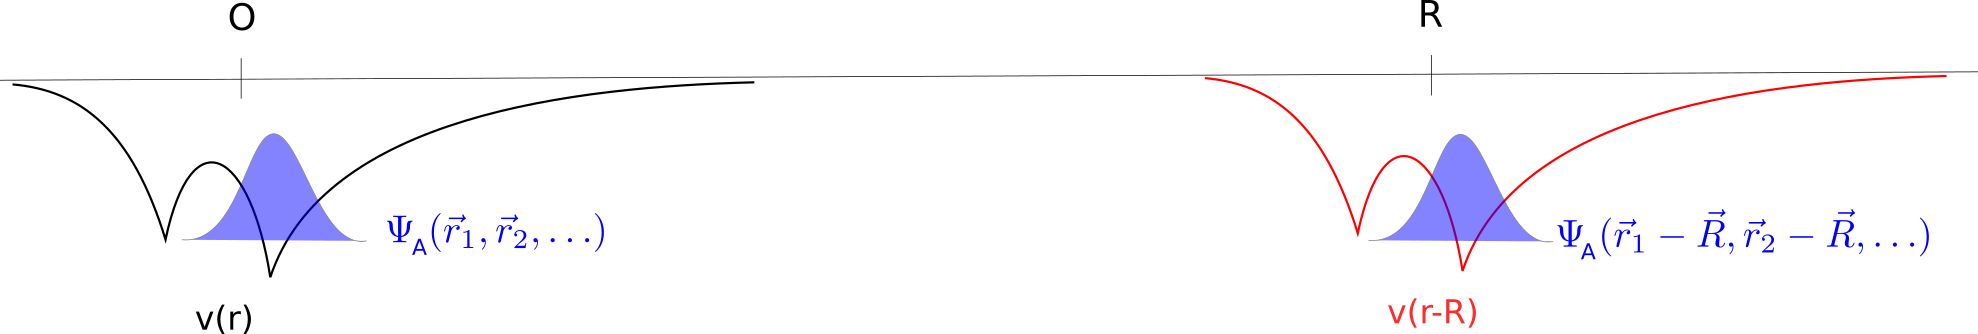
\includegraphics[width=0.9\linewidth]{figures/repeated_external_potential.png}
  \caption{\label{fig:repeated_external_potential} External potential of two identical molecules separated by a large distance $R$. The localized wavefunction in the left and right potential wells are identical except for the rigid shift.}
\end{figure}

$\mathbb{V}_{\vec{O}}^N$ is the subspace spanned by $N$ bound, electronic wavefunctions (not necessarily eigenstates) that are localized around the origin $\vec{O}$.
These wavefunctions decay exponentially with distance \cite{Katriel1980asymptotic}. $\mathbb{V}_{\vec{R}}^N$ is spanned by the same wavefunctions rigidly translated to the center $\vec{R}$. A subspace of twice the dimension is formed by combining the subspaces of the left and right molecules,
\begin{equation}
  \begin{split}
    \mathbb{V}^{2N} = \mathbb{V}^{N}_{\vec{O}} \cup \mathbb{V}^{N}_{\vec{R}} = \Span\Big\{ &
                  \Psi_1(\vec{r}_1,\vec{r}_2,\ldots),
                  \Psi_2(\vec{r}_1,\vec{r}_2,\ldots), \ldots,
                  \Psi_N(\vec{r}_1,\vec{r}_2,\ldots), \\
    &             \Psi_1(\vec{r}_1-\vec{R},\vec{r}_2-\vec{R},\ldots),
                  \Psi_2(\vec{r}_1-\vec{R},\vec{r}_2-\vec{R},\ldots), \ldots,
                  \Psi_N(\vec{r}_1-\vec{R},\vec{r}_2-\vec{R},\ldots) \Big\}.
  \end{split}
\end{equation}
Because of the large distance $R$, the transition densities between states localized at $\vec{O}$ and those at $\vec{R}$ vanish. The state densities and transition densities among the states localized on the same molecule are the same for both moleules except for a rigid shift. The matrix density for the combined subspace therefore consists of two blocks of size $N$, each:
\begin{equation}
  \m{D}^{(2N)}(\vec{r}) =
  \begin{pmatrix}
    \m{D}^{(N)}(\vec{r}) & 0 \\
    0 & \m{D}^{(N)}(\vec{r}-\vec{R})
  \end{pmatrix}
\end{equation}
As the distance between the two molecules is increased ($R \to \infty$), the matrix elements of the Hamiltonian vanishes, $\langle \Psi_{A} \vert \hat{H} \vert \Psi_{B} \rangle \to 0$, if the wavefunctions $\Psi_A$ and $\Psi_B$ are localized on different molecules. The matrix elements of the kinetic energy decrease exponentially, $\langle \Psi_{A} \vert \hat{T} \vert \Psi_{B} \rangle \propto \exp(-\alpha R)$, for the Coulomb operator the decrease is like $\langle \Psi_{A} \vert \hat{W} \vert \Psi_{B} \rangle \propto \frac{1}{R}$.
Therefore, in the limit $R \to \infty$, the universal part of the Hamiltonian in the subspace $\mathbb{V}^{(2 N)}$ is just block-diagonal, $\hat{H}^{(2N)}_0 = \hat{H}^{(N)} \oplus \hat{H}^{(N)}$. The projection of $\hat{H}_0$ into the combined subspace $\mathbb{V}^{(2N)}$ is a functional of the matrix density $\m{D}^{(2N)}$, and the Hamiltonians in the individual subspaces $\mathbb{V}^{(N)}_{\vec{O}}$ and $\mathbb{V}^{(N)}_{\vec{R}}$ are functionals of the matrix densities $\m{D}^{(N)}(\vec{r})$ and $\m{D}^{(N)}(\vec{r}-\vec{R})$, respectively. Furthermore the universal functional should be translationally invariant, so that $\mathcal{F}^{(N)}[\m{D}^{(N)}(\vec{r}-\vec{R})] = \mathcal{F}^{(N)}[\m{D}^{(N)}(\vec{r})] = \m{H}^{(N)}_0$. Therefore the following relation holds between the functionals $\mathcal{F}^{(2N)}$ and $\mathcal{F}^{(N)}$:
\begin{equation}
  \mathcal{F}^{(2N)}
  \left[
    \begin{pmatrix}
      \m{D}^{(N)}(\vec{r}) & 0 \\
      0 & \m{D}^{(N)}(\vec{r}-\vec{R})
    \end{pmatrix}
    \right]
  =
  \begin{pmatrix}
    \m{H}^{(N)}_{0} & 0 \\
    0 & \m{H}^{(N)}_{0}
  \end{pmatrix}
  =
  \begin{pmatrix}
    \mathcal{F}^{(N)}[\m{D}(\vec{r})] & 0 \\
    0 & \mathcal{F}^{(N)}[\m{D}(\vec{r})]
  \end{pmatrix} \label{eqn:relation_F2N_FN}
\end{equation}

The plan is to plug the functional Taylor expansion of Eqn.~\ref{eqn:functional_taylor_expansion} into Eqn.~\ref{eqn:relation_F2N_FN} in order to work out the relation between the functional $\mathcal{F}^{(2N)}$ and $\mathcal{F}^{(N)}$. A priori it is assumed that the functional could be different for different subspace dimensions. It will be shown that this is not the case. However, Eqn.~\ref{eqn:relation_F2N_FN} is not yet in a suitable form to compare the two functionals, since on its LHS the functional $\mathcal{F}^{(2N)}$ operates on a matrix density of dimension $2N$, while on the RHS the arguments of the functional $\mathcal{F}^{(N)}$ have dimension $N$. So we have to transform the expession in such a way, that $\mathcal{F}^{(2N)}$ operates on a matrix density of dimension $N$.
%%%

First some preliminaries.
The functional Taylor expansion involves integrations over three-dimensional space.
The three-dimensional space is partitioned into Voronoi polyhedra. Each point $\vec{r}$ is assigned to the closest molecule,
\begin{align}
  V_{\vec{O}} &= \{\vec{r}: \vert \vec{r} \vert < \vert \vec{r} - \vec{R} \vert \} \\
  V_{\vec{R}} &= \{\vec{r}: \vert \vec{r} - \vec{R} \vert \leq \vert \vec{r} \vert \} \\
  \mathbb{R}^3 &= V_{\vec{O}} \cup V_{\vec{R}}.
\end{align}
Integration over space is split into separate integrations over the Voronoi polyhedra,
\begin{equation}
 \int_{\mathbb{R}^3} \ldots d^3\!r = \int_{V_{\vec{O}}} \ldots d^3\!r + \int_{V_{\vec{R}}} \ldots d^3\!r.
\end{equation}
Since the wavefunctions are localized around the potential at either $\vec{O}$ or $\vec{R}$, there is no point in space where $\m{D}(\vec{r})$ and $\m{D}(\vec{r}-\vec{R})$ are simultaneously non-zero. So dependening on where the point $\vec{r}$ lies, the projection of the density operator in the subspace $\mathbb{V}^{2N}$ has only one non-zero block at the top or at the bottom:
\begin{equation}
  \m{D}^{(2N)}(\vec{r}) = \m{D}^{(N)}(\vec{r}) \oplus \m{D}^{(N)}(\vec{r}-\vec{R}) =
  \begin{cases}
    \m{D}^{(N)}(\vec{r}) \oplus 0 & \text{if } \vec{r} \in V_{\vec{O}} \\
    0 \oplus \m{D}^{(N)}(\vec{r}-\vec{R}) & \text{if } \vec{r} \in V_{\vec{R}} \label{eqn:D_split}
  \end{cases}
\end{equation}
Similarly we get for the trace,
\begin{equation}
  \tr\left(\m{D}^{(2N)}(\vec{r}) \right)
  =
  \tr\left(\m{D}^{(N)}(\vec{r}) \oplus \m{D}^{(N)}(\vec{r}-\vec{R}) \right)
  =
  \begin{cases}
    \tr(\m{D}(\vec{r})) & \text{if } \vec{r} \in V_{\vec{O}} \\
    \tr(\m{D}(\vec{r}-\vec{R}) & \text{if } \vec{r} \in V_{\vec{R}} \label{eqn:tr_split}
  \end{cases}
\end{equation}
If the functional should depend implicitly on the subspace dimension, the number of electronic states has to be expressed as a functional of the matrix density. One way to do this is
\begin{equation}
 \mathcal{N}(\vec{r}) = \tr\left\{ \m{D}(\vec{r}) \m{D}^{-1}(\vec{r}) \right\}.
\end{equation}
If at some point the matrix density does not have full rank and therefore is not invertible, the pseudinverse is used instead of the inverse. $\mathcal{N}(\vec{r})$ always equals the rank of the matrix density.
Since $\m{D}^{(2N)}(\vec{r})$ has at most rank $N$ (the number of wavefunctions that are simultaneously non-zero is at most $N$),
\begin{equation}
  \mathcal{N}^{(2N)}(\vec{r})
  =
  \begin{pmatrix}
    \mathcal{N}^{(N)}(\vec{r}) & \text{if } \vec{r} \in V_{\vec{O}} \\
    \mathcal{N}^{(N)}(\vec{r}-\vec{R}) & \text{if } \vec{r} \in V_{\vec{R}}. \label{eqn:N_split}
  \end{pmatrix}
\end{equation}

Now we write out the Taylor expansion and focus only on the term linear in $\m{D}^{(2N)}(\vec{r})$, but higher-order terms work the same way:

\begin{align}
  &\mathcal{F}^{(2N)}[\m{D}^{(2N)}(\vec{r})] = \int d^3\!r_1 ~ f^{(1)}\left(\vec{r}_1; \tr(\m{D}^{(2N)}(\vec{r}_1)), \mathcal{N}^{(2N)}(\vec{r}_1) \right) \m{D}^{(2N)}(\vec{r}_1) + \ldots \nonumber \\
    =& \int d^3\!r_1 ~ f^{(1)}\left(\vec{r}_1; \tr(\m{D}^{(2N)}(\vec{r}_1)), \mathcal{N}^{(2N)}(\vec{r}_1) \right)
    \begin{pmatrix}
      \m{D}^{(N)}(\vec{r}_1) & 0 \\
      0 & \m{D}^{(N)}(\vec{r}_1 - \vec{R})
    \end{pmatrix} + \ldots \nonumber \\
    =& \int_{V_{\vec{O}}} d^3\!r_1 ~ f^{(1)}\left(\vec{r}_1; \tr(\m{D}^{(N)}(\vec{r}_1)), \mathcal{N}^{(N)}(\vec{r}_1) \right)
    \begin{pmatrix}
      \m{D}^{(N)}(\vec{r}_1) & 0 \\
      0 & 0
    \end{pmatrix} \nonumber \\
    & + \int_{V_{\vec{R}}} d^3\!r_1 ~ f^{(1)}\left(\vec{r}_1; \tr(\m{D}^{(N)}(\vec{r}_1-\vec{R})), \mathcal{N}^{(N)}(\vec{r}_1-\vec{R}) \right)
    \begin{pmatrix}
      0 & 0 \\
      0 & \m{D}^{(N)}(\vec{r}_1-\vec{R})
    \end{pmatrix} + \ldots \nonumber \\
    =&
    \begin{pmatrix}
      \int_{\mathbb{R}^3} d^3\!r_1 ~ f^{(1)}\left(\vec{r}_1; \tr(\m{D}^{(N)}(\vec{r}_1)), \mathcal{N}^{(N)}(\vec{r}_1) \right) \m{D}^{(N)}(\vec{r}_1) + \ldots & 0 \\
      0 & \int_{\mathbb{R}^3} d^3\!r_1 ~ f^{(1)}\left(\ldots \right) \m{D}^{(N)}(\vec{r}_1-\vec{R}) + \ldots\\
    \end{pmatrix} \nonumber \\
    =&
    \begin{pmatrix}
      \mathcal{F}^{(2N)}[\m{D}^{(N)}(\vec{r})] & 0 \\
      0 & \mathcal{F}^{(2N)}[\m{D}^{(N)}(\vec{r})]
    \end{pmatrix} \label{eqn:relation_F2N_FN_same_dim}
\end{align}

In going from line 2 to 3 of Eqn.~\ref{eqn:relation_F2N_FN_same_dim}, the integration was split up and the corresponding cases from Eqns.~\ref{eqn:D_split},\ref{eqn:tr_split},\ref{eqn:N_split} were used inside each integration volume. In going from lines 3 and 4 to line 5, the integration range was extended again over the entire $\mathbb{R}^3$, since the respective integrands vanish on the additional volume. Finally, to get to the last line, we sum up the Taylor expansion again to obtain $\mathcal{F}^{(2N)}$ evaluated on the matrix density in the subspaces $\mathbb{V}_{\vec{O}}$ and $\mathbb{V}_{\vec{R}}$, respectively. As the universal functional has translational invariance, we can use $\mathcal{F}^{(2N)}[\m{D}^{(N)}(\vec{r}-\vec{R})] = \mathcal{F}^{(2N)}[\m{D}^{(N)}(\vec{r})]$.
Comparison of Eqn.~\ref{eqn:relation_F2N_FN_same_dim} with Eqn.~\ref{eqn:relation_F2N_FN} shows that
\begin{equation}
 \mathcal{F}^{(2N)}[\m{D}^{N}(\vec{r})] = \mathcal{F}^{(N)}[\m{D}^{N}(\vec{r})]
\end{equation}
for any matrix density $\m{D}^{(N)}(\vec{r})$ that decays exponentially with distance.
% [READ \cite{Katriel1980asymptotic} and \cite{Levy1984exact}, wavefunction and density of bound states should decay exponentially with distance]
Now the dimension of the argument is the same on both sides. The above equality suggests that the same universal functional applies to all subspace dimensions and one can drop the superscript and simply write $\mathcal{F}[\m{D}(\vec{r})]$. For $N=1$ it is equal to the ground-state kinetic and Hartree-exchange-correlation (Hxc) functionals,
\begin{equation}
 \mathcal{F}[\rho(\vec{r})] = T[\rho(\vec{r})] + E_{\text{Hxc}}[\rho(\vec{r})]
\end{equation}
However, deducing the exact multi-state functional from known ground-state kinetic-energy and Hartree-exchange-correlation functionals is not readily possible.
Even if one has a closed expression of a local functionals in term of $\rho(\vec{r})$,
it is not clear where $\rho(\vec{r})$ has to be replaced by the scalar $\tr(\m{D}(\vec{r}))$
and where by the matrix $\m{D}(\vec{r})$.
For $N=1$, all three are the same, i.e. $\rho(\vec{r}) = \tr(\m{D}(\vec{r})) = \m{D}(\vec{r})$.
Nevertheless ground-state functionals can give some guidance.

The next step is to find a multistate matrix density functional, that has the required transformation properties
 and reduces to a known ground state functional for $N=1$.

\subsection{An Approximate Matrix Functional}
\label{sec:approximate_lda_msdft}
The electronic Hamiltonian $\hat{H} = \hat{T} + \hat{W} + \hat{V}$ consists of
the kinetic energy $\hat{T} = \sum_{a=1}^{n} -\frac{1}{2} \nabla^2_a$,
the electron-electron repulsion $\hat{W} = \sum_{a < b}^{n} \frac{1}{\vert \hat{\vec{r}}_a - \hat{\vec{r}}_b \vert}$
and the external potential $\hat{V} = \sum_{a=1}^{n} v(\vec{r}_a)$, where $v(\vec{r})$ usually is the electron-nuclear attraction.
While the projection of the external potential into any subspace is trivially a functional of the matrix density of that subspace,
\begin{equation}
 V[\m{D}(\vec{r})]_{IJ} = \langle \Psi_I \vert \hat{V} \vert \Psi_J \rangle = \int d^3r ~ v(\vec{r}) D_{IJ}(\vec{r}),
\end{equation}
the functionals for $\hat{T}$ and $\hat{W}$ have to be approximated. The kinetic energy multistate functional
will be derived from the Thomas-Fermi and von-Weizs\"{a}cker ground state functionals. The electron-electron repulsion
is split into a Hartree-like direct term, a Dirac-like exchange term, a correlation-like term based on Chachiyo's fit to
the correlation energy of the homogeneous electron gas and a self-interaction correction for the core electrons. Let us start
with the electron-electron repulsion.

\subsubsection{Electron Repulsion Functional}
The matrix element of the electron repulsion operator, $\sum_{a < b}^{n} 1/\vert \vec{r}_a - \vec{r}_b \vert$,
between two electronic states $\Psi_I$ and $\Psi_J$ with $n$ electrons is
\begin{equation}
 W_{IJ} = 
\int dx_1 \int dx_2 \ldots \int dx_{n} ~ \Psi_{I}^*(\vec{x}_1, \vec{x}_2, \ldots, \vec{x}_n)
\sum_{a < b}^{n} \frac{1}{\vert \vec{r}_a - \vec{r}_b \vert}
\Psi_{J}(\vec{x}_1, \vec{x}_2, \ldots, \vec{x}_n), \label{eqn:electron_repulsion_exact}
\end{equation}
where $\vec{x}_a = (\vec{r}_a, \sigma_a)$ are the spatial and spin coordinates of electron $a$.
According to the theorem by Lu and Gao \cite{Lu2022JPCL}, which is the multi-state equivalent of the Hohenberg-Kohn theorem,
$W_{IJ}$ is a functional of the matrix density $\m{D}(\vec{r})$.
In the Thomas-Fermi-Dirac (TFD) model \cite[chapter 6]{ParrYangBook} the electron-electron repulsion consists of the
classical electrostatic energy of the total electronic charge $\rho = \rho^{\alpha} + \rho^{\beta}$ ($\alpha$ denotes spin up, $\beta$ spin down) and the exchange energy 
\begin{equation}
U_{ee}^{\text{TFD}}[\rho] = \frac{1}{2} \int \int' \frac{\rho(\vec{r}) \rho(\vec{r}')}{\vert \vec{r}-\vec{r}' \vert} d^3r d^3r'
 - 2^{1/3} C_x \int [\rho^{\alpha}(\vec{r})]^{4/3} + [\rho^{\beta}(\vec{r})]^{4/3} ~ d^3r.
\end{equation}
%The value of the prefactor $C_x = 0.7937$ is taken from the "Gaussian" approximation in Eqn.~(6.5.25)
The value of the prefactor $C_x = 0.7386$ is taken from the Dirac's approximation \cite{Dirac1930} (see also Eqn.~(6.1.20)
of chapter 6 of the textbook by Parr \& Yang \cite{ParrYangBook}), so that $2^{1/3} C_x = 0.93058$
(same as Eqn.(35) in Ref.~\cite{Perdew1981}).
Since $W_{IJ}[\m{D}]$ is an \emph{analytic} matrix functional,
the Thomas-Fermi-Dirac functional for the ground state can be turned into a multistate functional by keeping the same functional form
and replacing $\rho$ with the spin-traced matrix density $\m{D} = \m{D}^{\alpha} + \m{D}^{\beta}$. This process is not unique, since the single-state
functional does not contain the complete information about the multi-state functional.
\footnote{For instance, the density product $\rho(\vec{r}') \rho(\vec{r})$ could become
either the matrix product $\m{D}(\vec{r}) \m{D}(\vec{r}')$
or $\tr(\m{D}(\vec{r})) \m{D}(\vec{r}')$, since for a single state both options are identical.}
However, the simplest choice is to replace scalar multiplication with matrix multiplication, so that the multistate extension
of the TFD electron repulsion energy becomes
\begin{equation}
W^{\text{TFD}}[\m{D}^{\alpha},\m{D}^{\beta}]_{IJ} = 
\frac{1}{2} \sum_{K} \int \int' \frac{D_{IK}(\vec{r}) D_{KJ}(\vec{r}')}{\vert \vec{r}' - \vec{r} \vert} ~ d^3r d^3r'
- 2^{1/3} C_x \int [\m{D}^{\alpha}]^{4/3}(\vec{r})_{IJ} + [\m{D}^{\beta}]^{4/3}(\vec{r})_{IJ} ~ d^3r
\end{equation}
Because of the requirement that $W[\m{D}]_{IJ}$ is an analytic matrix functional, the Hartree-like term 
\begin{equation}
\m{J}[\m{D}] = \frac{1}{2} \int \int' \frac{\m{D}(\vec{r}) \m{D}(\vec{r}')}{\vert \vec{r} - \vec{r}' \vert} \label{eqn:Hartree_term}
\end{equation}
contains a matrix product that mixes the electron density of a single state,
$D_{II}(\vec{r})$ with the transition densities $D_{IJ}(\vec{r}')$ ($I \neq J$).
The electrostatic energy of a single excited state, which has a classical interpretation, cannot be calculated in
isolation. It depends on the transition densities, which have no classical analogue.
Only if the transition densities to other states in the selected subspace vanish everywhere, can the state be
treated in isolation. 
%This situation might occur for a doubly excited state that is dark. [THe state is dark because the transition dipole moment vanishes, but the density does not have to be zero everywhere!!!]
%Multistate density functional theory thus provides a justification for the applicability of the $\Delta SCF$ method.

% Exchange-energy of uniform electron gas
The exchange-like term in the local density approximation (LDA) \cite[6.1.20]{ParrYangBook},
\begin{equation}
  \m{K}^{\text{LDA}}[\m{D}] = C_x \int (\m{D}(\vec{r}))^{4/3} ~ d^3r, \label{eqn:exchange_term_lda}
\end{equation}
or in the local spin density approximation (LSDA) \cite[8.2.16]{ParrYangBook},
\begin{equation}
  \m{K}^{\text{LSDA}}[\m{D}^{\alpha},\m{D}^{\beta}] = 2^{1/3} C_x \int (\m{D}^{\alpha}(\vec{r}))^{4/3} + (\m{D}^{\beta}(\vec{r}))^{4/3} ~ d^3r, \label{eqn:exchange_term_lsda}
  \end{equation}
involves a fractional matrix power of the matrix density, $(\m{D}^{\alpha})^{4/3}$.
It is important to stress that this is different from applying the function $\bullet^{4/3}$ to
each element of the matrix. The best way to actually compute a matrix function such as the fractional power,
is to first do a spectral decomposition of the matrix density at each point in space. Let
$\m{\Lambda}(\vec{r}) = \Diag\left(\lambda_1(\vec{r}),\lambda_2(\vec{r}),\ldots,\lambda_N(\vec{r}) \right)$ be the diagonal
matrix of eigenvalues of $\m{D}(\vec{r})$, which is a function of the point in space $\vec{r}$. The corresponding orthonormalized
eigenvectors are the columns of the unitary matrix $\m{U}(\vec{r})$ satisfying $\m{U}^{\dagger}(\vec{r}) \m{U}(\vec{r}) = \m{I}_{N \times N}$, $\forall \vec{r}$.
Then the eigendecomposition of $\m{D}(\vec{r})$ is
\begin{equation}
 \m{D}(\vec{r}) = \m{U}(\vec{r}) \m{\Lambda}(\vec{r}) \m{U}^{\dagger}(\vec{r})
\end{equation}
Note that eigenvalues and eigenvectors are functions of space. And the fractional matrix power is 
\begin{equation}
  \m{D}^{4/3}(\vec{r}) = \m{U}(\vec{r}) \m{\Lambda}^{4/3}(\vec{r}) \m{U}^{\dagger}(\vec{r}).
\end{equation}
In general any analytic scalar function $f : \mathbb{C} \mapsto \mathbb{C}$ can be converted into an analytic
matrix function $\m{F}[\m{D}]: \mathbb{C}^{N \times N} \mapsto \mathbb{C}^{N \times N}$ by applying $f$ to
the eigenvalues of $\m{D}$. 
Actually applying the ground state exchange functional element-wise is not even possible, since the transition density $D_{IJ}(\vec{r})$
can be negative. For negative arguments the fractional power is not uniquely defined. This problem does not occur for the fractional matrix
power, since the matrix density is positive definite, so that all eigenvalues are positive everywhere.

% Correlation energy of uniform eletron gas
Let us move on to the correlation energy.
The Chachiyo functional \cite{Chachiyo2016} is a simple and elegant parametrization of the correlation energy per electron.
It recovers the high-density limit and fits the quantum Monte-Carlo results of Ceperley and Alder ~\cite{Ceperley1980} rather well.
In terms of the Wigner-Seitz radius $r_s=\left(4 \pi /3 \rho\right)^{-1/3}$ the correlation energy per particle is given
by $\epsilon_{\text{corr}}(\rho) = a \log(1 + b r_s^{-1} + b r_s^{-2})$. Since $\epsilon_{\text{corr}}$ is an analytic function of the electron density
it can be turned into a multistate functional by retaining the
functional form and replacing the scalar density argument $\rho=\rho^{\alpha}+\rho^{\beta}$
with the matrix density $\m{D}=\m{D}^{\alpha}+\m{D}^{\beta}$. Considering only the paramagnetic part of the correlation energy,
the multistate extension of the Chachiyo correlation functional (Eqn.~8 in Ref.~\cite{Chachiyo2016}) can be written in the following form:
\begin{equation}
 \m{C}^{\text{LDA}}[\m{D}] = \int a \log\left( \Id + b_1 \m{D}^{1/3}(\vec{r}) + b_2 \m{D}^{2/3}(\vec{r}) \right) \m{D}(\vec{r}) ~ d^3r
 \label{eqn:LDA_correlation_energy}
\end{equation}
with the parameters
\begin{align}
 a &= \frac{\log(2)-1}{2 \pi^2} = -0.01554534543482745 \\
 b &= 20.4562557 \quad \text{(paramagnetic case)} \\
 b_1 &= \left(4 \pi /3 \right)^{1/3} b = 32.975319597703546 \\
 b_2 &= \left(4 \pi /3 \right)^{2/3} b = 53.155949872619715.
\end{align}
The integrand of Eqn.~\ref{eqn:LDA_correlation_energy}, the correlation energy density,
is calculated by diagonalizing $\m{D}$,
applying the function $f(D) = a \log(1 + b_1 D^{1/3} + b_2 D^{2/3}) D$ to the eigenvalues
and transforming the result back from the eigenbasis to the original basis.
For a single electronic state Eqn.~\ref{eqn:LDA_correlation_energy} reduces to the correlation energy
of the local density approximation.
This functional only evaluates the paramagnetic part of the correlation
energy, the spin polarization is assumed to be zero.
For closed-shell molecules the diagonal elements of the matrix density are not spin-polarized, however
the transition densities usually have a large spin-polarization. However, it is not obvious how to turn the spin
polarization $\zeta = (\rho^{\alpha} - \rho^{\beta})/\rho$ into a matrix functional. With spin polarization the
matrix functional would have to depend on two matrix densities, $\m{D}^{\alpha}+\m{D}^{\beta}$ and $\m{D}^{\alpha}-\m{D}^{\beta}$,
which do not commute.
The correlation energy of the uniform electron gas is always negative. For medium
and low densities ($0.5 \leq r_s \leq 10.0$), the ratio of ferromagnetic to paramagnetic
correlation energy is approximately $1.1$, see Fig.~\ref{fig:correlation_energy_paramagnetic_fs_ferromagnetic} in the Supporting Information (SI).
So by neglecting the difference between paramagnetic and ferromagnetic correlation
we incur and error of approximately 10\%.

The Hartree term (the direct part of the Coulomb energy) accounts for most of the electron repulsion, both in the diagonal
and the off-diagonal elements of the electron repulsion matrix.
It is almost an order of magnitude larger than the exchange-correlation term (the indirect part).
The functional form of the Hartree term (Eqn.~\ref{eqn:Hartree_term}) for the off-diagonal elements
can be justified qualitatively as follows:
Suppose for simplicity that the wavefunctions $\Psi_{I},\Psi_{J},\ldots$
in the electronic subspace are Hartree products built from a set of orthonormal orbitals $\phi_{a}(\vec{r})$.
The electrons are assumed to be spinless and distinguishable.
All wavefunctions have $n-1$ orbitals ($\phi_1,\ldots,\phi_{n-1}$) in common
and differ only in the last orbital ($\phi_I$ or $\phi_J$ etc.).
\begin{align}
 \Psi_I &= \phi_1(\vec{r}_1) \phi_2(\vec{r}_2) \cdots \phi_{n-1}(\vec{r}_{n-1}) \phi_{I}(\vec{r}) \\
 \Psi_J &= \underbrace{\phi_1(\vec{r}_1) \phi_2(\vec{r}_2) \cdots \phi_{n-1}(\vec{r}_{n-1})}_{\text{"inactive"}} \phi_{J}(\vec{r})
\end{align}
The diagonal and off-diagonal parts of the matrix density for these states are
\begin{equation}
 D_{II}(\vec{r}) = \sum_{1 \leq a \leq n-1} \vert \phi_a(\vec{r}) \vert^2 + \vert \phi_I(\vec{r}) \vert^2
\end{equation}
and
\begin{equation}
  D_{IJ}(\vec{r}) = \phi^*_I(\vec{r}) \phi_J(\vec{r}) \quad \quad I \neq J,
\end{equation}
respectively. The matrix element of the electron repulsion operator between two different states is
\begin{equation}
  \begin{split}
W_{IJ} &= \int d^3r_1 \ldots \int d^3r_n ~ 
\Psi^*_{I}(\vec{r}_1,\vec{r}_2,\ldots,\vec{r}_n)
\sum_{1 \leq a < b \leq n} \frac{1}{\vert \vec{r}_a - \vec{r}_b \vert}
\Psi_{J}(\vec{r}_1,\vec{r}_2,\ldots,\vec{r}_n) \\
&= \int d^3r_1 \ldots \int d^3r_n ~ 
\sum_{1 \leq a < b \leq n} \frac{
  \vert \phi_1(\vec{r}_1) \vert^2 \ldots \vert \phi_{n-1}(\vec{r}_{n-1}) \vert^2 \phi^*_I(\vec{r}_n) \phi_J(\vec{r}_n)
  }{\vert \vec{r}_a - \vec{r}_b \vert} \\
&= \int d^3r_1 \int d^3r_2 \left(\sum_{1 \leq a \leq n-1} \vert \phi_a(\vec{r}_1) \vert^2 \right)
  \frac{1}{\vert \vec{r}_1 - \vec{r}_2 \vert}
  D_{IJ}(\vec{r}_2) \label{eqn:Hartree_exact_electron_repulsion}
  \end{split}
\end{equation}
The last equality follows because all terms that involve an integral over $\vec{r}_n$ vanish since $\phi_I$ and $\phi_J$ are orthogonal.
So $W_{IJ}$ is the electrostatic interaction of the transition density with the density of the "inactive" orbitals
that are shared by all electronic states. On the other hand, the Hartree-term in Eqn.~\ref{eqn:Hartree_term} gives
\begin{align}
 J[\m{D}]_{IJ} &= \frac{1}{2} \int d^3r_1 \int d^3r_2 \sum_K \frac{D_{IK}(\vec{r}_1) D_{KJ}(\vec{r}_2)}{\vert \vec{r}_1 - \vec{r}_2 \vert} \nonumber \\
 &= \int \int \frac{1}{2} 
  \left( D_{II}(\vec{r}_1) + D_{JJ}(\vec{r}_1) \right)
  \frac{1}{\vert \vec{r}_1 - \vec{r}_2 \vert}
  D_{IJ}(\vec{r}_2) +
  \frac{1}{2} \sum_{K \neq I,J} \int \int D_{IK}(\vec{r}_1) \frac{1}{\vert \vec{r}_1 - \vec{r}_2 \vert} D_{KJ}(\vec{r}_2)
  \label{eqn:Hartree_term_offdiagonal}
\end{align}
In going from the first to the second line, the terms where $K$ is equal to $I$ or $J$ were separated out.
The first term in Eqn.~\ref{eqn:Hartree_term_offdiagonal} differs from the exact electron repulsion (Eqn.~\ref{eqn:Hartree_exact_electron_repulsion})
only by the spurious electrostatic interaction of $D_{IJ}$ with $\frac{1}{2} (\vert \phi_I \vert^2 + \vert \phi_J \vert^2)$
(I think this interaction is called "ghost interaction", see text below Eqn.(14) in \cite{Pastorczak2014}).
The additional second term in Eqn.~\ref{eqn:Hartree_term_offdiagonal} involves the electrostatic interaction
between transition densities of $I$ and $K$. It is much smaller than the first, since densitities have magnitudes
on the order of $n$ (number of electron), while transition densities are on the order of $<1$.
The additional term is needed to ensure that $\m{J}[\m{D}(\vec{r})]$ is a matrix functional of $\m{D}$ and transforms as
$\m{J}[\m{U} \m{D}(\vec{r}) \m{U}^{-1}] = \m{U} \m{J}[\m{D}(\vec{r})] \m{U}^{-1}$ under a basis transformation of the electronic states.

For $I=J$ the second term in Eqn.~\ref{eqn:Hartree_term_offdiagonal} is positive, so that
$J[\m{D}]_{II}$ is larger than the electrostatic repulsion of the state density $D_{II}$ alone. The trace of the Hartree-like
matrix functional is larger than the sum of the Hartree energies of the individual states,
\begin{equation}
 \tr(\m{J}[\m{D}]) \ge \sum_{I=1}^{N} \frac{1}{2} \int \int' \frac{D_{II}(\vec{r}) D_{II}(\vec{r}')}{\vert \vec{r} - \vec{r}' \vert}. \label{eqn:J_inequality}
\end{equation}
However, in the electron repulsion without correlation, $\m{J}[\m{D}] - \m{K}^{\text{LDA}}[\m{D}]$,
this larger direct electron repulsion is partly compensated for by the
exchange part of the indirect electron repulsion $\m{K}^{\text{LDA}}$, which on average is larger than the
exchange energies of the individual electronic states,
\begin{equation}
 \tr(\m{K}^{\text{LDA}}[\m{D}]) = C_x \int d^3r \tr(\m{D}^{4/3}(\vec{r})) \ge \sum_{I=1}^N C_x \int d^3r ~ D_{II}(\vec{r})^{4/3}. \label{eqn:K_inequality}
\end{equation}
This is a result of Klein's inequality \cite{wiki:Kleins_inequality} \cite{Ruelle1969statistical} and is proven in section \ref{sec:Kleins_inequality} of the SI.
The correlation energy is left out in the comparison since it is usually an order of magnitude smaller than the exchange energy.

\subsubsection{Self-Interaction Error of Core Electrons}
% see section 8.3 in Parr & Yang
Many failures of the local spin density approximation can be attributed to the self-interaction error. \cite{Perdew1981}
The largest part of the deviation between the exact electron repulsion $\m{W}$ and
the MSDFT approximation $\m{J}[\m{D}]-\m{K}^{\text{LDA}}[\m{D}] + \m{C}^{\text{LDA}}[\m{D}]$ does not depend on the geometry.
This suggests that it is due to the core electrons, which do not participate in the bonding.
It is known that in the core regions the self-interaction errors are particularly large (see section D in Ref. \cite{Tsuneda2014}).
We have to subtract the unphysical interaction of a core electron with itself. An electron in a 1s spin-up ($\alpha$) core orbital $\phi^{\alpha}_{1s}(\vec{r})$
contributes to the DFT electron repulsion the spurious interaction of the density $\rho^{\alpha}_{1s}(\vec{r}) = \vert \phi^{\alpha}_{1s}(\vec{r})\vert^2$
with itself. There is a Hartree-like contribution,
\begin{equation}
J[\rho^{\alpha}_{1s}] = \frac{1}{2} \int \int' \frac{\rho^{\alpha}_{1s}(\vec{r}) \rho^{\alpha}_{1s}(\vec{r}')}{\vert \vec{r} - \vec{r}' \vert},
\end{equation}
an exchange-like contribution,
\begin{equation}
-K^{\text{LSDA}}[\rho^{\alpha}_{1s}] = - 2^{1/3} C_x \int \rho^{\alpha}_{1s}(\vec{r})^{4/3},
\end{equation}
and a correlation-like contribution,
\begin{equation}
C[\rho^{\alpha}_{1s}] = \int \rho^{\alpha}_{1s}(\vec{r}) \epsilon_{\text{corr}}(\rho^{\alpha}_{1s}(\vec{r})),
\end{equation}
that have to be subtracted from the diagonal elements $W_{II}[\m{D}]$.
This completely removes a single core electron's repulsion with itself.
The off-diagonal elements $W_{IJ}[\m{D}]$, $I \neq J$, do not suffer from the self-intersection problem.
The self-interaction energies from different elements (except the very light ones like hydrogen, lithium etc.) are added.
Since core orbitals are doubly occupied, a factor of two appears.
The self-interaction correction (SIC) is supposed to cancel the self-interaction error (SIE), so there is a minus sign in front:
\begin{equation}
\text{SIC} = - \sum_{c}^{\text{core orbs.}} 2 \left(
  \frac{1}{2} \int \int' \frac{\rho_{c}(\vec{r}) \rho_{c}(\vec{r}')}{\vert \vec{r} - \vec{r}' \vert}
  - 2^{1/3} C_x \int \rho_c(\vec{r})^{4/3}
  + \int \rho_c(\vec{r}) \epsilon_{\text{corr}}(\rho_c(\vec{r}))
 \right)
\end{equation}
This self-interaction correction is not a functional of the matrix density. Like its ground state counterpart,
the multistate 
LDA-like
%Thomas-Fermi-Dirac-like 
functional is too simplistic to cancel the self-interaction, so that a correction
outside of the MSDFT formalism has to be employed.

The self-interaction correction is a constant that only depends on the elemental composition of the molecule, but not
on the geometry and is the same for all electronic states. So the final expression for the matrix elements of the electron repulsion 
in the subspace of the lowest few electronic states is
\begin{equation}
W[\m{D}]_{IJ} = J[\m{D}]_{IJ} - K^{\text{LDA}}[\m{D}]_{IJ} + C^{\text{LDA}}[\m{D}]_{IJ} + \text{SIC} ~ \delta_{IJ}. \label{eqn:electron_repulsion_msdft}
\end{equation}

\subsection{Kinetic Energy Functional}
The kinetic energy of a nearly-homogeneous electron gas ($\rho \approx \text{const}$, $\nabla \rho \approx 0$) is
\begin{equation}
T[\rho] = T_{\text{TF}}[\rho] + \frac{1}{9} T_{\text{vW}}[\rho], \label{fig:kinetic_energy_TFvW_ground_state}
\end{equation}
with the 
Thomas-Fermi (TF) functional,
\begin{equation}
T_{\text{TF}}[\rho(\vec{r})] = \frac{3}{10} (3 \pi^2)^{2/3} \int \rho(\vec{r})^{5/3} ~ d^3\!r,
\end{equation}
which is exact for the free, non-interacting electron gas, and the von Weizs\"{a}cker (vW) correction,
\begin{equation}
T_{\text{vW}}[\rho(\vec{r})] = \frac{1}{8} \int \frac{ \vert \nabla \rho(\vec{r}) \vert^2}{\rho(\vec{r})} ~ d^3\!r, \label{eqn:Tvw_ground_state}
\end{equation}
which yields the exact kinetic energy for a single electron.
The factor $\frac{1}{9}$ in the Thomas-Fermi-von-Weizs\"{a}cker functional of Eqn.~\ref{fig:kinetic_energy_TFvW_ground_state}
stems from the conventional gradient expansion to second order around the homogeneous electron gas limit. \cite[section 6.7]{ParrYangBook}

The generalization of the Thomas-Fermi functional to multiple
electronic states is obtained by
replacing the density $\rho(\vec{r})$ by the matrix density $\m{D}(\vec{r})$ and taking the fractional matrix power $\m{D}^{5/3}(\vec{r})$,
\begin{equation}
  T_{\text{TF}}[\m{D}(\vec{r})]_{IJ} = \frac{3}{10} (3 \pi^2)^{2/3} \int \left[ \m{D}(\vec{r})^{5/3} \right]_{IJ} ~ d^3\!r.
\end{equation}

The von-Weizs\"{a}cker functional depends on both the density and its gradient,
which turn into non-commuting matrices $\m{D}$ and $\nabla \m{D}$ in the multistate case.
The ground state functional of Eqn.~\ref{eqn:Tvw_ground_state} does not determine the order of the factors uniquely.
If the matrix inverse is placed symmetrically between the two gradients, which form a scalar product, the
multistate von-Weizs\"{a}cker functional becomes
\begin{equation}
  T_{\text{vW}}[\m{D}(\vec{r})]_{IJ} = \int d^3\!r ~ \frac{1}{8} \sum_{K} \sum_{L} \nabla D_{IK}(\vec{r}) \left(\m{D}^{-1}(\vec{r}) \right)_{KL} \nabla D_{KL}(\vec{r}).
  \label{eqn:von_Weizsaecker_many_electrons}
\end{equation}
This is not the only conceivable extension. One could also use the gradient of the matrix square root of $\m{D}$,
\begin{equation}
T_{\text{vWsqrt}}[\m{D}(\vec{r})]_{IJ} 
= \frac{1}{8} \int d^3\!r ~ \sum_{K}^N \nabla (D^{1/2})_{IK}(\vec{r}) \nabla (D^{1/2})_{KJ}(\vec{r}).
\label{eqn:vW_ms_extension_matrix_square_root}
\end{equation}
Since $\nabla \m{D}$ and $\m{D}$ do not commute,
$\nabla \m{D}^{1/2} \cdot \nabla \m{D}^{1/2} \neq \nabla \m{D} \m{D}^{-1} \nabla \m{D}$,
unlike in the single-state case, where $\left(\nabla \sqrt{\rho}\right)^2 = \nabla \rho^2 / \rho$.
For the small systems studied, equations \ref{eqn:von_Weizsaecker_many_electrons} and \ref{eqn:vW_ms_extension_matrix_square_root}
give slightly different results, but it is not clear which one is superior.
In particular neither functional is exact for 1-electron systems.

The kinetic functional that will be used in the Results section is taken as
\begin{equation}
T[\m{D}(\vec{r})] = T_{\text{TF}}[\m{D}(\vec{r})] + \frac{1}{9} T_{\text{vW}}[\m{D}(\vec{r})]. \label{eqn:kinetic_energy_msdft}
\end{equation}

\subsection{Incorporating Exact Constraints}
\label{sec:exact_constraints}
Exact constraints can help to narrow down the form of a multistate functional.
This will be illustrated for the von-Weizs\"{a}cker functional.
The von-Weizs\"{a}cker functional $T[\rho]$ gives the exact kinetic energy for a single electron wavefunction $\phi(\vec{r}) = \sqrt{\rho(\vec{r})}$.
However, neither Eqn.~\ref{eqn:von_Weizsaecker_many_electrons} nor Eqn.~\ref{eqn:vW_ms_extension_matrix_square_root} yield the correct
matrix elements of the kinetic energy operator for a one-electron system.
In the following a kinetic energy functional is derived that reduces to the von-Weizs\"{a}cker functional for $N=1$ and gives the
exact kinetic energy matrix for single-electron wavefunctions.

Let the single particle wavefunctions be denoted as $\phi_I(\vec{r})$. With the help of Gauss' law
the matrix elements of the kinetic energy operator between states $I$ and $J$ can be expressed as
\begin{equation}
    T_{IJ} = -\frac{1}{2} \int d^3\!r ~ \phi^*_I \nabla^2 \phi_J
    = \int d^3\!r ~ \frac{1}{2} (\nabla \phi^*_I)\cdot (\nabla \phi_J). \label{eqn:kinetic_energy_1e}
\end{equation}
For a single-electron system, the matrix density is just the product of the wavefunctions (the density matrix),
\begin{equation}
 D_{IJ}(\vec{r}) = \phi^*_I(\vec{r}) \phi_J(\vec{r}).
\end{equation}
Note that for wavefunctions of a single electron
\begin{equation}
 \sum_{K=1}^{N} D_{IK} D_{KJ} = \phi^*_I \sum_{K} \phi_{K} \phi^*_{K} \phi_J = \tr(\m{D}) D_{IJ},
\end{equation}
however, this relation is not true for matrix densities of multi-electron systems.

To derive the von-Weizs\"{a}cker kinetic energy functional one has to assume that all wavefunctions are real, so that $D_{IJ} = \phi_I \phi_J$.
Now consider
\begin{equation}
\begin{split}
  & \sum_K (\nabla D_{IK}) \cdot (\nabla D_{KJ})
  = \sum_K (\nabla \phi_I \phi_K + \phi_I \nabla \phi_K)\cdot (\nabla \phi_K \phi_J + \phi_K \nabla \phi_J) \\
  =&
  (\sum_K \phi_K \phi_K) \nabla \phi_I \cdot \nabla \phi_J +
  \sum_K (\nabla \phi_K \cdot \nabla \phi_K) \phi_I \phi_J +
  \sum_K (\nabla \phi_I \cdot \nabla \phi_K) \phi_K \phi_J +
  \sum_K \phi_I \phi_K (\nabla \phi_K \cdot  \nabla \phi_J) \\
  =& \tr(\m{D}) (\nabla \phi_I \cdot \nabla \phi_J) + D_{IJ} \sum_{K} (\nabla \phi_K \cdot \nabla \phi_K) + \sum_K (\nabla \phi_I \cdot \nabla \phi_K) D_{KJ}
  + \sum_K D_{IK} (\nabla \phi_K \cdot \nabla \phi_J)
\end{split}
\end{equation}
The kinetic energy density $T_{IJ}(\vec{r}) = \frac{1}{2} \nabla \phi_I(\vec{r}) \cdot \nabla \phi_J(\vec{r})$ (the integrand in Eqn.~\ref{eqn:kinetic_energy_1e}) appears on the right hand side multiple times. Rewriting the previous equation in terms of $T_{IJ}(\vec{r})$ gives
\begin{equation}
T_{IJ}(\vec{r}) = \underbrace{\frac{1}{2} \frac{\sum_K \nabla D_{IK} \cdot \nabla D_{KJ}}{\tr(\m{D})}}_{C_{IJ}(\vec{r})} - \underbrace{\frac{D_{IJ}}{\tr(\m{D})}}_{R_{IJ}(\vec{r})} \sum_K T_{KK}(\vec{r}) - \sum_{K} T_{IK}(\vec{r}) \underbrace{\frac{D_{KJ}}{\tr(\m{D})}}_{R_{KJ}(\vec{r})} - \sum_{K} \underbrace{\frac{D_{IK}}{\tr(\m{D})}}_{R_{IK}(\vec{r})} T_{KJ}(\vec{r}) \label{eqn:kinetic_density_multistate}
\end{equation}
For a single electronic state ($N=1$), we get $C = \frac{1}{2} (\nabla \rho)\cdot (\nabla \rho) / \rho$, $R = 1$ and the above equation reduces to
\begin{equation}
t_{\text{vW}}(\vec{r}) = \frac{1}{2} \frac{\nabla \rho \cdot \nabla \rho}{\rho} - 3 t_W(\vec{r})
\end{equation}
or
\begin{equation}
t_{\text{vW}}(\vec{r}) = \frac{1}{8} \frac{\nabla \rho(\vec{r}) \cdot \nabla \rho(\vec{r})}{\rho(\vec{r})}, \label{eqn:von_Weizsaecker_ked}
\end{equation}
which is the kinetic energy density of the familiar von-Weizs\"{a}cker functional \cite{Weizsacker1935},
\begin{equation}
  T_{\text{vW}}[\rho] = \int t_{\text{vW}}[\rho](\vec{r}) d^3\!r  \label{eqn:von_Weizsaecker_functional}.
\end{equation}
For $N > 1$ Eqn.~\ref{eqn:kinetic_density_multistate} is a system of linear equations,
\begin{equation}
 T_{IJ}(\vec{r}) = C_{IJ} - R_{IJ} \sum_K T_{KK} - \sum_K T_{IK} R_{KJ} - \sum_K R_{IK} T_{KJ}
\end{equation}
that has to be solved for $T_{IJ}(\vec{r})$ at each point $\vec{r}$.
To solve the linear system, $T_{IJ}(\vec{r})$ is treated as a vector in $\mathbb{R}^{N \times N}$ and the equation is rewritten as
\begin{equation}
T_{IJ}(\vec{r}) = C_{IJ}(\vec{r}) + \sum_{K,L=1}^{N} \mathcal{K}_{IJ,KL}(\vec{r}) T_{KL}(\vec{r}) \label{eqn:CplusKT}
\end{equation}
This equation has the form $\vec{T} = \vec{C} + \mathcal{K} \vec{T}$, which can be solved for the vector $\vec{T} = (1 - \mathcal{K})^{-1} \vec{C}$.
By writing Eqn.~\ref{eqn:CplusKT} as
\begin{equation}
T_{IJ}(\vec{r}) = C_{IJ}(\vec{r}) + \sum_{K,L} \left\{ - R_{IK}(\vec{r}) \delta_{LJ} - \delta_{IK} R_{LJ}(\vec{r}) - R_{IJ}(\vec{r}) \delta_{KL} \right\} \vec{T}_{KL}(\vec{r}) \label{eqn:vonWZ_matrix_equation}
\end{equation}
we see that the matrix $\mathcal{K} \in \mathbb{R}^{N^2 \times N^2}$ is
\begin{equation}
 \mathcal{K}_{IJ,KL} = - R_{IK}(\vec{r}) \delta_{LJ} - \delta_{IK} R_{LJ}(\vec{r}) - R_{IJ}(\vec{r}) \delta_{KL}
\end{equation}
Under the assumption $\lvert \mathcal{K} \rvert < 1$, $(1 - \mathcal{K})^{-1}$ can be written as a geometric series
\begin{equation}
 (1 - \mathcal{K})^{-1} = \sum_{k=0}^{\infty} \mathcal{K}^{k}
\end{equation}
so that
\begin{equation}
\vec{T} = \sum_{k=0}^{\infty} \mathcal{K}^{k} \vec{C} = \vec{C} + \sum_{k=1}^{\infty} \mathcal{K}^{k} \vec{C} \label{eqn:solution_geometric_series}
\end{equation}
To prove $\lvert \mathcal{K} \rvert < 1$, we have to show that $R_{IJ} < 1$. This follows from
\begin{equation}
D_{IJ}(\vec{r}) = \phi_I(\vec{r}) \phi_J(\vec{r}) \leq \max_{K} \phi_K(\vec{r}) \phi_K(\vec{r}) \leq \sum_K \phi_K(\vec{r}) \phi_K(\vec{r}) = \tr(\m{D})
\end{equation}
Eqn.~\ref{eqn:solution_geometric_series} demonstrates that the kinetic energy density obtained by solving Eqn.~\ref{eqn:vonWZ_matrix_equation} is indeed a functional of the matrix density $\m{D}$. The first term of the series \ref{eqn:solution_geometric_series} is
\begin{equation}
\begin{split}
  (\mathcal{K} \vec{C})_{IJ} &= -\sum_{K} R_{IK} C_{KJ} - \sum_{K} C_{IK} R_{KJ} - R_{IJ} \sum_K C_{KK} \\
   &= - (\m{R} \m{C} + \m{C} \m{R})_{IJ} - R_{IJ} \tr(\m{C}).
\end{split}
\end{equation}
Since $\m{R}$ and $\m{C}$ are analytic matrix functionals of $\m{D}$, i.e. $\m{R}[\m{U} \m{D} \m{U}^{-1}] = \m{U} \m{R}[\m{D}] \m{U}^{-1}$ and similarly for $\m{C}$,
we conclude that $\mathcal{K} \vec{C}$ and $\mathcal{K} (\mathcal{K} \vec{C})$ etc. are analytic matrix functionals, which only depend on $\m{D}(\vec{r})$, $\nabla \m{D}(\vec{r})$ and the scalar invariant $\tr(\m{D})$, as well.

Although for $N=1$ it reduces to the simple expression in Eqn.~\ref{eqn:von_Weizsaecker_functional},
the \emph{multistate} von-Weizsaecker functional of Eqn.~\ref{eqn:solution_geometric_series} is an infinite series. 
This suggests that trying to guess the functional form of a matrix density functional from a known ground state functional
with non-commuting terms (such as functionals from the generalized gradient approximation (GGA) family)
will in general not be crowned with success.
Taking only the first two terms of the infinite series, the kinetic energy functional reads
\begin{equation}
\begin{split}
  \m{T}_{\text{vW1e}}[\m{D}(\vec{r})] =& \int \m{C} ~ d^3\!r  - \int \left(\m{R} \m{C} + \m{C} \m{R} + \tr(\m{C}) \m{R} \right) d^3\!r  + \ldots \\
  =& \int \frac{1}{2} \tr(\m{D})^{-1} (\nabla \m{D} \cdot \nabla \m{D}) ~ d^3\!r \\
  & - \int \frac{1}{2} \tr(\m{D})^{-2} \left[ \m{D} (\nabla \m{D} \cdot \nabla \m{D}) + (\nabla \m{D} \cdot \nabla \m{D}) \m{D} + \tr(\nabla \m{D} \cdot \nabla \m{D}) \m{D} \right] ~ d^3\!r + \ldots .
\end{split}
\label{eqn:TvW1e}
\end{equation}
In practice $\m{T}_{\text{vW1e}}[\m{D}(\vec{r})]$ is determined by solving Eqn.~\ref{eqn:CplusKT} for
each grid point and then integrating the kinetic energy density numerically.

Figures \ref{fig:vW_kinetic_energy_HMI} and \ref{fig:vW_kinetic_energy_LiH} compare the kinetic energy densities
of two von-Weizs\"{a}cker-like functionals $\m{T}_{\text{vW}}$ (Eqn.~\ref{eqn:von_Weizsaecker_many_electrons})
and $\m{T}_{\text{vW1e}}$ (Eqn.~\ref{eqn:TvW1e}) with the exact results
computed with full configuration interaction as implemented in the PySCF \cite{Sun2020} software package. Clearly \textbf{vW1e} is exact for 1-electron systems
but significantly understimates the kinetic energy density for multiple electrons.
The \textbf{vW} functional works well in the vicinity of the nuclei where the electron density is high, but less so in the bonding regions.
But both functionals reproduce the transition density accurately.
More exact conditions are needed to constrain the kinetic energy functional.
%Reproducing the exact kinetic energy matrix on density matrices belonging to one-particle wavefunctions is not 

\begin{figure}[h!]
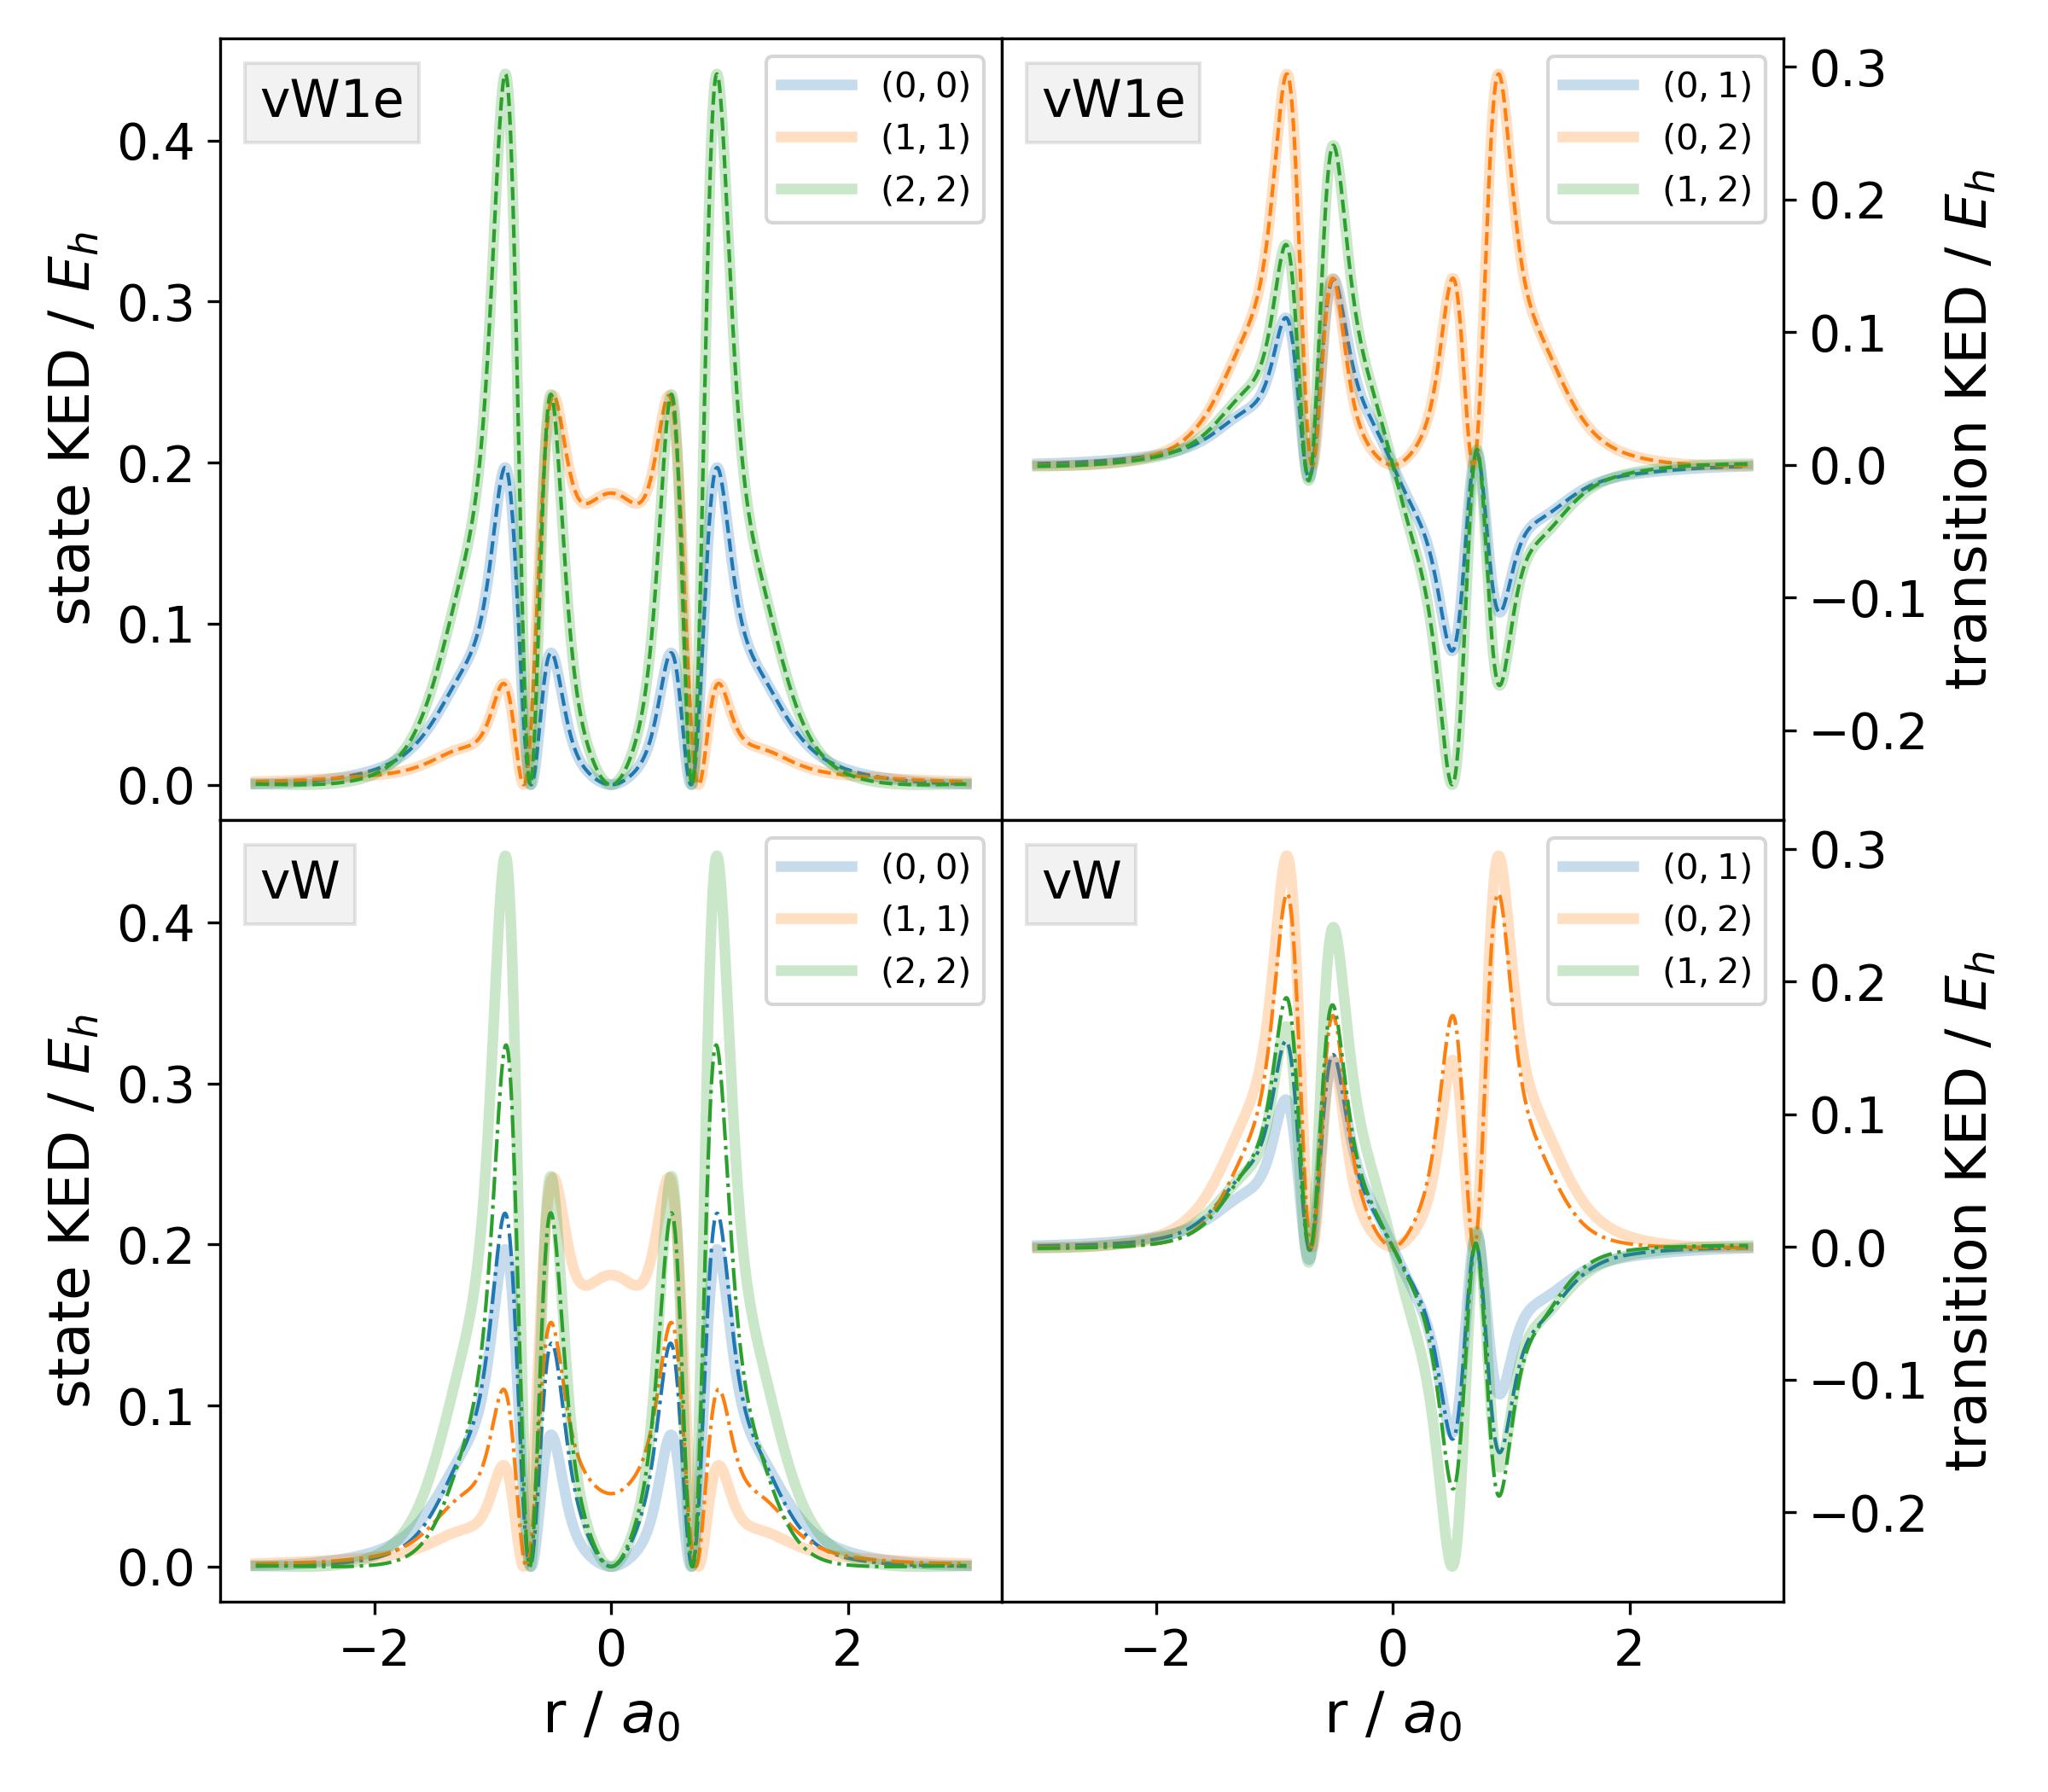
\includegraphics[width=0.8\textwidth]{figures/vW_kinetic_energy_HMI.png}
\caption{\textbf{1-electron system.} Cut through the kinetic energy density (KED) of hydrogen molecular ion, H$_2^+$, along the bond axis for the lowest three electronic states $I,J=0,1,2$. Solid, thick lines represent the exact kinetic energy density computed as ${T_{IJ} = -\frac{1}{2} \int \nabla \phi_I(\vec{r}) \cdot \nabla \phi_J(\vec{r})}$ from a calculation with the 6-31g basis set using PySCF. Dashed, thin lines are the KEDs computed with approximate kinetic energy functionals according to Eqn.~\ref{eqn:solution_geometric_series} (\textbf{vW1e}) and Eqn.~\ref{eqn:von_Weizsaecker_many_electrons} (\textbf{vW}). Diagonal state KED's $(I,I)$ are shown on the left, transition KED's $(I,J)$ on the right.}
\label{fig:vW_kinetic_energy_HMI}
\end{figure}

\begin{figure}[h!]
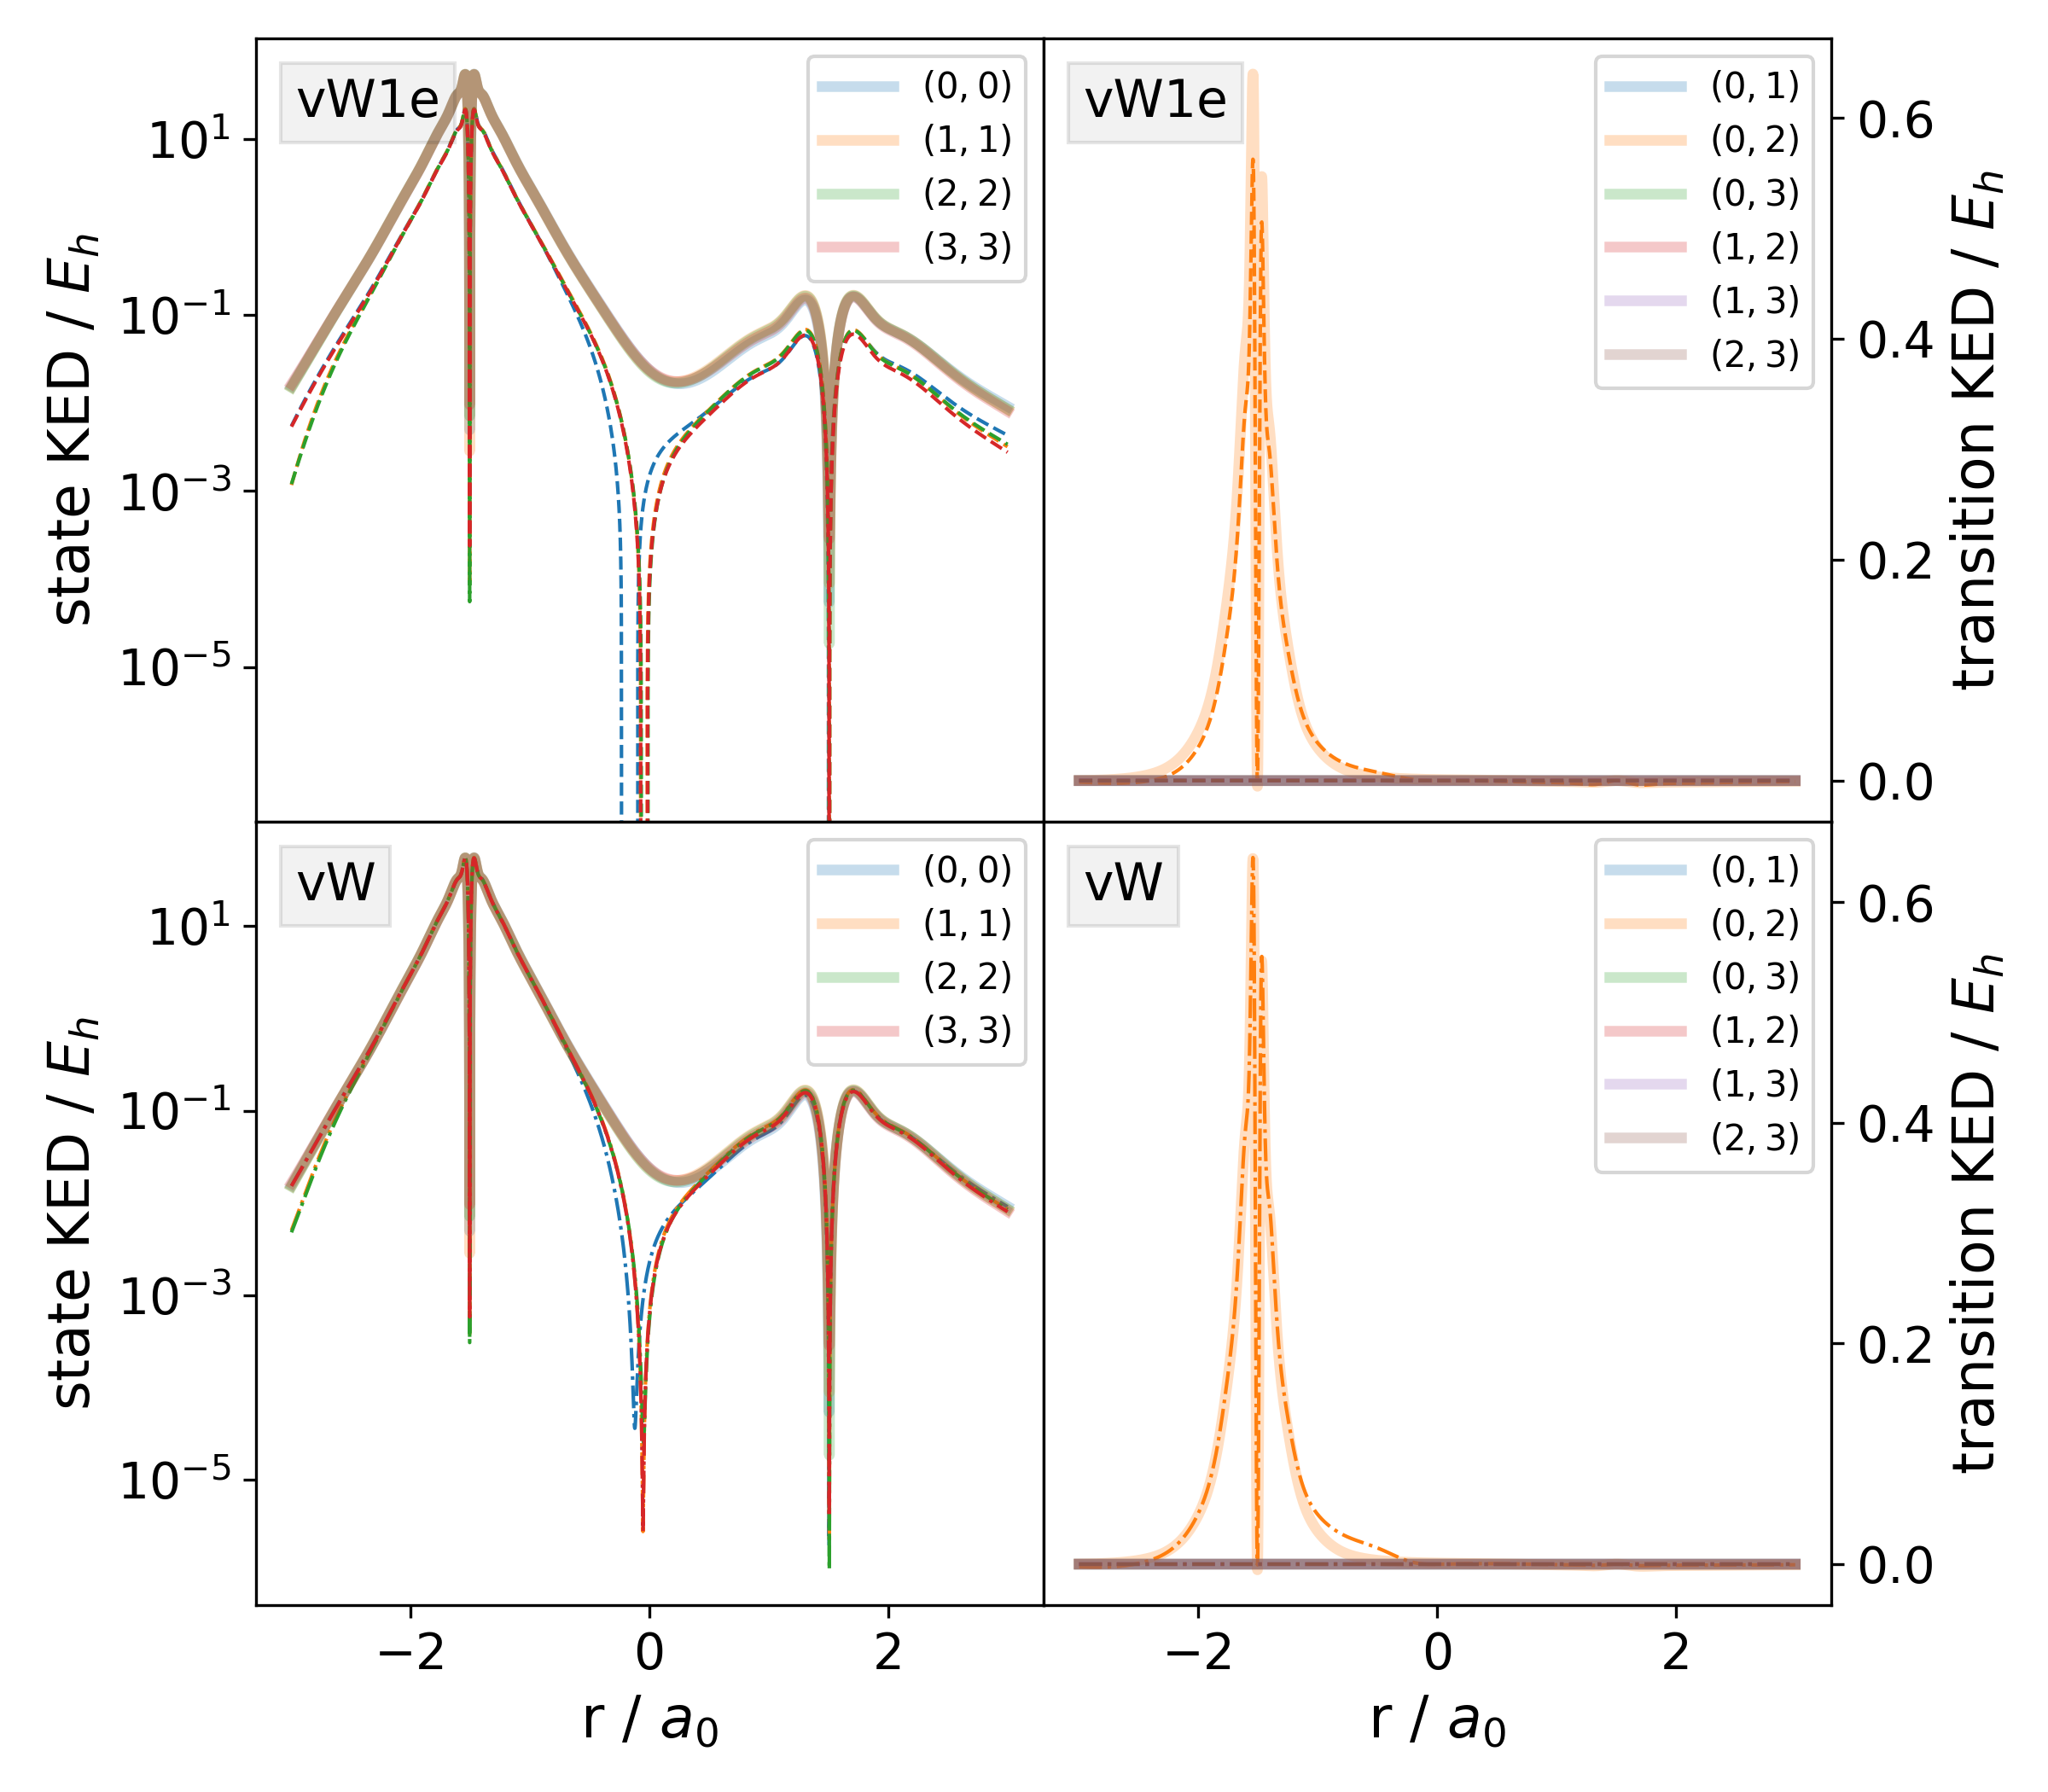
\includegraphics[width=0.8\textwidth]{figures/vW_kinetic_energy_LiH-lda.png}
\caption{\textbf{Lithium hydride.} Cut through the kinetic energy density (KED) of lithium hydride, LiH, along the bond axis for the lowest four electronic states $I,J=0,1,2,3$. Solid, thick lines represent the exact kinetic energy density from a FCI/6-31g calculation using PySCF. Dashed, thin lines are the KEDs computed with approximate kinetic energy functionals according to Eqn.~\ref{eqn:solution_geometric_series} (\textbf{vW1e}) and Eqn.~\ref{eqn:von_Weizsaecker_many_electrons} (\textbf{vW}). Diagonal state KED's $(I,I)$ are shown on the left (log), transition KED's $(I,J)$ on the right.}
\label{fig:vW_kinetic_energy_LiH}
\end{figure}

\FloatBarrier

\subsection{Excited States of the Homogeneous Electron Gas}
\label{sec:heg_msdft}
Except for the von-Weizs\"{a}cker correction all multistate functionals presented above are local density approximations.
The LDA expressions are derived from the homogeneous electron gas, where the density is a constant,
and are transferred to inhomogeneous systems.
Assuming that the density changes little within a small volume element $d^3\!r$,
the homogeneous electron gas expressions are applied to the density in each volume element. Summing
over all space gives the total energy. The LDA is exact for the ground state of the homogeneous electron gas,
but what about the multistate version of LDA? Is it exact for the excited states of the homogeneous electron gas?
And how do the lowest excited state of the homogeneous electron gas look like?

In order to maintain the validity of the LDA, the excited state wavefunctions have to be constants, too.
One can construct a homogeneous wavefunction with higher kinetic energy than the ground state by removing electrons
below the Fermi level and putting them into plane wave states above the Fermi level. \cite{Hemanadhan2010}
However, no matter how the electrons are distributed in k-space, the electron density will not change
since $\vert e^{\imath \vec{k} \cdot \vec{r}} \vert = 1$ for any $\vec{\vec{k}}$.
Therefore the diagonal elements of the matrix density are the same constant $D_{II}(\vec{r}) = \rho = \frac{n}{V}$
(number of electrons $n$ per volume $V$) for all states $I$.
However, the states become distinguishable when the transition densities are taken into account.
The transition densities are non-zero only between states that differ at most in the occupation of two plane-wave orbitals.
Let us assume that in the transition from the state $I$ to $J$, the wave vector of one electron is changed from
$\vec{k}_I$ to $\vec{k}_J$. Then the transition density is
$D_{IJ}(\vec{r}) = \frac{1}{\sqrt{V}} e^{\imath (\vec{k}_J - \vec{k}_I) \cdot \vec{r}}$.
However, there is a problem. The homogeneous electron gas does not have a gap between the ground state and the first excited state.
Also, since the homogeneous electron gas is of infinite size, the states form a continuum. Of course, one could pick out a subspace of $N$
electronic states and construct the matrix density. 
However, the matrix functional gives the exact Hamiltonian matrix only for the lowest $N$ electronic states.
For a random set of electronic states there is no guarantee that $\m{F}[\m{D}] + \int v(\vec{r}) \m{D}(\vec{r}) ~ d^3\!r$
maps their matrix density to the corresponding Hamiltonian matrix.
The only thing we know is that the average energy of those states will be larger than the average energy
of the same number of lowest-energy states. For a continuous spectrum the variational minimization of the subspace energy is not possible.
These considerations suggest that MSDFT is only applicable to bounds states of finite systems, which have a discrete spectrum
so that a matrix representation is adequate.

\subsection{Lower Bounds}
\label{sec:lower_bounds}
When searching for approximate density functionals, lower bounds on the kinetic energy and the exchange-correlation energy
are very useful. In the multistate density functional theory, the subspace expectation value of the energy is minimized
(Eqn.~(13) in Ref.~\cite{Lu2022JPCL}), which is the state-averaged (or MS for \emph{multistate}) energy,
\begin{equation}
  E_{\text{MS}}[\m{D}] = \frac{1}{N} \sum_{I=1}^{N} \mathcal{H}_{II}[\m{D}]
  = \frac{1}{N} \sum_{I=1}^{N} \left( \mathcal{F}_{II}[\m{D}] + \int d^3r ~ v(\vec{r}) D_{II}(\vec{r}) \right).
\end{equation}
Therefore one has to bound $\frac{1}{N} \tr(\mathcal{F}[\m{D}])$ from below rather than finding bounds of
the individual matrix elements $\mathcal{F}_{IJ}[\m{D}]$. The lower bounds for the average kinetic and electron repulsion energies
will be treated separately.

\subsubsection{Lower Bound of Kinetic Energy}
The kinetic energy of a single wavefunction is bounded from below by the von-Weiz\"{a}cker kinetic energy functional.
The proof for this inequality can be found below theorem 1.1 of Ref.~\cite{Lieb2002}. Applying this bound individually
to each electronic state in the subspace and averaging over states, one obtains a lower bound on the subspace kinetic energy,
\begin{equation}
 \frac{1}{N} \sum_{I=1}^{N} T_{II} \ge \frac{1}{N} \int d^3r ~ \frac{1}{8} \sum_{I=1}^{N} \frac{\vert \nabla D_{II}(\vec{r}) \vert^2}{D_{II}(\vec{r})}.
 \label{eqn:lower_bound_kinetic_sum_over_states}
\end{equation}
However, while the left hand side is a subspace invariant, i.e. it does not change under a basis transformation of the vectors in the subspace,
the right hand side is not. It is possible to find a bound on the average kinetic energy that is almost as tight but also is a subspace invariant.
The derivation proceeds in analogy with theorem 1.1 of Ref.~\cite{Lieb2002}. It is assumed that the $n$-electron wavefunctions are antisymmetric and orthonormal.
The wavefunctions in the subspace are put into an $N$-dimensional vector
$\vec{\Psi}(\vec{x}_1,\ldots,\vec{x}_n) = \left(\Psi_1(\vec{x}_1,\ldots,\vec{x}_n), \ldots, \Psi_N(\vec{x}_1,\ldots,\vec{x}_n)\right)$. One then defines
a scalar product on this vector space,
\begin{equation}
\langle \vec{\Psi}, \vec{\Phi} \rangle({\color{red} \vec{r}_1}) = \sum_{I=1}^{N} \sum_{\sigma_1=\uparrow,\downarrow} \int dx_2 \int dx_3 \cdots \int dx_n
  \Psi_I^*({\color{red} \vec{r}_1},\sigma_1;\vec{x}_2,\ldots,\vec{x}_n)
  \Phi_I({\color{red} \vec{r}_1},\sigma_1;\vec{x}_2,\ldots,\vec{x}_n),
\end{equation}
which sums over all electronic states $I=1,\ldots,N$ and integrates over all spatial and spin coordinates $\vec{x}_i = (\vec{r}_i,\sigma_i)$ for $i=2,\ldots,n$
except for the spatial coordinates ${\color{red} \vec{r}_1}$
of the first electron. The scalar product is therefore a function of $\vec{r}_1$. The integral over all coordinates except for $\vec{r}_1$ is abbreviated
by the symbol $\int^{\dagger} \ldots := \sum_{\sigma_1=\uparrow,\downarrow} \int dx_2 \int dx_3 \cdots \int dx_n \ldots$ ~.
Since the electrons are indistinguishable, it does not matter which electronic coordinate is left out in the integral.
The remaining electronic coordinate is denoted by $\vec{r} = \vec{r}_1$.
Since $\langle \vec{\Psi},\vec{\Psi} \rangle = n \sum_{I} D_{II}(\vec{r})$,
the gradient of the sum of the electron densities with respect to the remaining electron coordinate can be expressed as a scalar product,
\begin{equation}
  \begin{split}
 \sum_I \nabla D_{II}(\vec{r}) &= n \sum_I \int^{\dagger} \nabla \Psi_I^* \Psi_I + n \sum_I \int^{\dagger} \Psi_I^* \nabla \Psi_I \\
  &= n \langle \nabla \vec{\Psi}, \vec{\Psi} \rangle + n \langle \vec{\Psi}, \nabla \vec{\Psi} \rangle, \\
  \end{split}
\end{equation}
which is bounded from above by the triangle inequality,
\begin{equation}
  \begin{split}
\left\vert \sum_I \nabla D_{II}(\vec{r}) \right\vert &=
\left\vert n \langle \nabla \vec{\Psi}, \vec{\Psi} \rangle + n \langle \vec{\Psi}, \nabla \vec{\Psi} \rangle \right\vert \\
& \leq n \vert \langle \nabla \vec{\Psi}, \vec{\Psi} \rangle \vert + n \vert \langle \vec{\Psi}, \nabla \vec{\Psi} \rangle \vert \\
&= 2 n \vert \langle \nabla \vec{\Psi}, \vec{\Psi} \rangle \vert. \label{eqn:triangle_inequality}
  \end{split}
\end{equation}
$\vert \langle \nabla \vec{\Psi}, \vec{\Psi} \rangle \vert$ is bounded by the Cauchy-Schwarz inequality,
\begin{equation}
  \begin{split}
  \vert \langle \nabla \vec{\Psi}, \vec{\Psi} \rangle \vert^2 &\leq
  \vert \langle \nabla \vec{\Psi}, \nabla \vec{\Psi} \rangle \vert \vert \langle \vec{\Psi}, \vec{\Psi} \rangle \vert \\
  &= \sum_I \int^{\dagger} \vert \nabla \Psi_I \vert^2 ~ \frac{1}{n} \sum_{J} D_{JJ}. \label{eqn:Cauchy_Schwarz}
  \end{split}
\end{equation}
In $n \int^{\dagger} \frac{1}{2} \vert \nabla \Psi_I \vert^2$ one recognizes the kinetic energy density $T_{II}(\vec{r})$ of the electronic state $I$.
Combining the inequalities \ref{eqn:triangle_inequality} and \ref{eqn:Cauchy_Schwarz} one gets
\begin{equation}
  \begin{split}
 \vert \sum_I \nabla D_{II}(\vec{r}) \vert^2 &\leq 4 n^2 \left(\sum_I \int^{\dagger} \vert \nabla \Psi_I \vert^2 \right) \left( \frac{1}{n} \sum_J D_{JJ} \right) \\
 &= 8 \left( \sum_I n \int^{\dagger} \frac{1}{2} \vert \nabla \Psi_I \vert^2 \right) \sum_J D_{JJ} \\
 &= 8 \sum_I T_{II}(\vec{r}) \sum_J D_{JJ}(\vec{r}),
  \end{split}
\end{equation}
which can be rearranged into
\begin{equation}
 \sum_I T_{II}(\vec{r}) \geq \frac{1}{8} \frac{\vert \sum_I \nabla D_{II}(\vec{r}) \vert^2}{\sum_J D_{JJ}(\vec{r})}.
\end{equation}
This inequality holds at very point in space. Dividing both sides by the number of states, expressing the right hand side in terms of the subspace
density $\rho_{V} = \frac{1}{N} \tr(\m{D}) = \frac{1}{N} \sum_I D_{II}(\vec{r})$, and integrating over the remaining electron coordinate,
the lower bound on the average kinetic energy of the subspace becomes
\begin{equation}
\frac{1}{N} \sum_{I=1}^{N} \langle \Psi_I \vert \sum_{i=1}^{n} \left(-\frac{1}{2} \nabla_i^2 \right) \vert \Psi_I \rangle
\geq \frac{1}{8} \int \frac{\left\vert \nabla \rho_{V}(\vec{r}) \right\vert^2}{\rho_{V}(\vec{r})} d^3r.
\label{eqn:lower_bound_kinetic_subspace_invariant}
\end{equation}
This lower bound is a functional of the subspace density $\rho_{V}(\vec{r})$ and is therefore an invariant property of the subspace.
Table \ref{tbl:lower_bounds_kinetic_energy} compares the exact average kinetic energy of the lowest 4 states for a few small molecules
with the lower bounds according to Eqn.~\ref{eqn:lower_bound_kinetic_sum_over_states}
and Eqn.~\ref{eqn:lower_bound_kinetic_subspace_invariant}, respectively.
For one-electron systems the bound of Eqn.~\ref{eqn:lower_bound_kinetic_sum_over_states} is exact. For molecules with many electrons,
both bounds are very close to each other, with the invariant bound of Eqn.~\ref{eqn:lower_bound_kinetic_subspace_invariant} slightly
less tight than that of Eqn.~\ref{eqn:lower_bound_kinetic_sum_over_states}. Overall the bounds are not tight enough to be very useful.


%%%%%%%%%%%%%%%%%%%%%% AUTO-GENERATE LATEX CODE (format_latex_table.py) %%%%%%%%%%%%%%%%%%%%%%%%%%%%%%%%%%%%%%%
\sisetup{
round-mode = places,
round-precision = 3,
scientific-notation = fixed,
fixed-exponent = 0,
zero-decimal-to-integer
}

\begin{table}
\begin{tabular}{
  SSSSS
  }
    \toprule
 {Molecule} & {Basis} & {Bound Eqn.~\ref{eqn:lower_bound_kinetic_Lieb}} & {Bound Eqn.~\ref{eqn:lower_bound_kinetic_invariant}} & {Exact}\\
\midrule
{H} & {6-31g} & 1.143235 & 0.823160 & 1.143235 \\
{H (large basis set)} & {aug-cc-pvtz} & 0.292371 & 0.150067 & 0.292371 \\
{H$_2^+$} & {6-31g} & 1.250525 & 0.767747 & 1.250525 \\
{H$_2$} & {6-31g} & 1.146228 & 0.973287 & 1.434804 \\
{Li} & {6-31g} & 7.206488 & 7.146008 & 7.384005 \\
{LiH} & {6-31g} & 7.669143 & 7.613865 & 7.976373 \\
{water} & {sto-3g} & 57.577183 & 57.446115 & 75.553086 \\
{O$_2$} & {sto-3g} & 113.211488 & 113.163189 & 146.582754 \\
{NO} & {sto-3g} & 99.286293 & 99.202325 & 126.551376 \\
{He} & {6-31g} & 4.157342 & 3.462193 & 4.649976 \\
{Ne} & {6-31g} & 90.150973 & 90.096788 & 130.121379 \\
\bottomrule
\end{tabular}

\caption{
\label{tbl:lower_bounds_kinetic_energy}
The exact subspace kinetic energy $\frac{1}{N} \sum_{I=1}^{N} T_{II}$ (\textbf{Exact}) is bounded from below by
$\frac{1}{N} \frac{1}{8} \sum_{I=1}^{N} \int \frac{\vert \nabla D_{II} \vert^2}{D_{II}}$
(\textbf{Bound Eqn.~\ref{eqn:lower_bound_kinetic_Lieb}}) and by the subspace invariant
$\frac{1}{8} \int \frac{\vert \nabla \rho_V \vert^2}{\rho_V}$
(\textbf{Bound Eqn.~\ref{eqn:lower_bound_kinetic_invariant}})
The exact wavefunctions for the $N=4$ lowest excited states ($N=2$ for hydrogen atom with small basis sets)
are calculated with full configuration interaction for a few small atoms and molecules.
All energies are in Hartree.}
\end{table}
%%%%%%%%%%%%%%%%%%%%%% END OF AUTO-GENERATE LATEX CODE %%%%%%%%%%%%%%%%%%%%%%%%%%%%%%%%%%%%%%%%%%
    


\subsubsection{Lower Bound of Electron Repulsion Energy}
A lower bound on the Coulomb energy of an arbitrary wavefunction
(not limited to Fermionic wavefunctions or those that are eigenstates of the Hamiltonian) in terms of
its charge density was proven by Lieb \cite{Lieb1979} and later improved upon by Lieb and Oxford \cite{Lieb1981}.
Applying the Lieb-Oxford bound to each electronic state separately and averaging over all $N$ states in the subspace
yields a bound on the average electron repulsion,
\begin{equation}
\frac{1}{N} \sum_{I=1}^{N} \langle \Psi_{I} \vert \sum_{i < j}^{n} \frac{1}{\vert \vec{r}_i - \vec{r}_j \vert} \vert \Psi_{I} \rangle
\geq \frac{1}{N} \sum_{I} \left( \frac{1}{2} \int \int' \frac{D_{II}(\vec{r}) D_{II}(\vec{r}')}{\vert \vec{r} - \vec{r}' \vert}
 - c_{\text{LO}} \int D_{II}(\vec{r})^{4/3} \right) \label{eqn:lieb_oxford_bound_sum_over_states} 
\end{equation}
with $c_{\text{LO}} = 1.68$ \cite{Lieb1981}. The right hand side of the inequality is not a subspace invariant, but this can be
remedied. A note at the end of the article by Lieb and Oxford \cite{Lieb1981} mentions that their inequality holds not only for pure states
but also for density matrices. The ensemble density matrix $\frac{1}{N} \sum_{I=1}^{N} \vert \Psi_I \rangle \langle \Psi_I \vert$, in which all
states have equal weights, gives rise to the subspace density $\rho_V(\vec{r})$. Invoking the Lieb-Oxford inequality for this ensemble
density matrix leads to a lower bound that is a functional of $\rho_V$ and therefore an invariant of the subspace,
\begin{equation}
  \frac{1}{N} \sum_{I=1}^{N} \langle \Psi_{I} \vert \sum_{a < b}^{n} \frac{1}{\vert \vec{r}_a - \vec{r}_b \vert} \vert \Psi_{I} \rangle
  \geq \frac{1}{2} \int \int' \frac{\rho_V(\vec{r}) \rho_V(\vec{r}')}{\vert \vec{r} - \vec{r}' \vert}
   - c_{\text{LO}} \int \rho_V(\vec{r})^{4/3}. \label{eqn:lieb_oxford_bound_subspace_invariant} 
\end{equation}
A detailed proof is given in section \ref{sec:lieb_oxford_bound_electron_repulsion} of the SI.

Table \ref{tbl:lower_bounds_electron_repulsion} compares the lower bounds of Eqns.~\ref{eqn:lieb_oxford_bound_sum_over_states} and
\ref{eqn:lieb_oxford_bound_subspace_invariant} with the exact average electron repulsion in the subspace. Both bounds are very similar,
but neither bound is strictly larger than the other. For some of the example molecules (e.g. He and Li), the subspace invariant
bound (Eqn.~\ref{eqn:lieb_oxford_bound_subspace_invariant}) is slightly larger,
whereas for water the sum over states bound (Eqn.~\ref{eqn:lieb_oxford_bound_sum_over_states}) is the larger one.


%%%%%%%%%%%%%%%%%%%%%% AUTO-GENERATE LATEX CODE (format_latex_table.py) %%%%%%%%%%%%%%%%%%%%%%%%%%%%%%%%%%%%%%%
\sisetup{
round-mode = places,
round-precision = 3,
scientific-notation = fixed,
fixed-exponent = 0,
zero-decimal-to-integer
}

\begin{table}
\begin{tabular}{
  SSSSS
  }
    \toprule
 {Molecule} & {Basis} & {SoS bound} & {Inv bound} & {Exact}\\
 & &  {Eqn.~\ref{eqn:lieb_oxford_bound_sum_over_states}} & {Eqn.~\ref{eqn:lieb_oxford_bound_subspace_invariant}} & \\
\midrule
{H} & {6-31g} & -0.213648 & -0.196269 & -0.000000 \\
{H (large basis set)} & {aug-cc-pvtz} & -0.109252 & -0.082824 & -0.000000 \\
{H$_2^+$} & {6-31g} & -0.204365 & -0.177504 & 0.000000 \\
{H$_2$} & {6-31g} & -0.023957 & -0.012915 & 0.536442 \\
{Li} & {6-31g} & 0.535950 & 0.550383 & 2.203327 \\
{LiH} & {6-31g} & 1.226790 & 1.234905 & 3.145189 \\
{water} & {sto-3g} & 28.633169 & 28.628061 & 38.119322 \\
{O$_2$} & {sto-3g} & 67.423964 & 67.422036 & 84.658835 \\
{NO} & {sto-3g} & 57.450087 & 57.447869 & 72.826637 \\
{He} & {6-31g} & -0.085329 & -0.060348 & 0.959691 \\
\bottomrule
\end{tabular}

\caption{
\label{tbl:lower_bounds_electron_repulsion}
The exact subspace electron repulsion energy
$\frac{1}{N} \sum_{I=1}^{N} \langle \Psi_I \vert \frac{1}{2} \sum_{i \neq j} \frac{1}{\vert \vec{r}_i - \vec{r}_j \vert} \vert \Psi_I \rangle$
(\textbf{Exact}) is bounded from below by
the \textbf{S}um \textbf{O}ver \textbf{S}tates bound $\frac{1}{N} \frac{1}{8} \sum_{I=1}^{N} \int \frac{\vert \nabla D_{II} \vert^2}{D_{II}}$
(\textbf{SoS bound} Eqn.~\ref{eqn:lieb_oxford_bound_sum_over_states}) and by the subspace \textbf{Inv}ariant bound
$\frac{1}{8} \int \frac{\vert \nabla \rho_V \vert^2}{\rho_V}$
(\textbf{Inv bound} Eqn.~\ref{eqn:lieb_oxford_bound_subspace_invariant})
The exact wavefunctions for the $N=4$ lowest excited states ($N=2$ for hydrogen atom with small basis sets)
are calculated with full configuration interaction for a few small atoms and molecules.
All energies are in Hartree.}
\end{table}
%%%%%%%%%%%%%%%%%%%%%% END OF AUTO-GENERATE LATEX CODE %%%%%%%%%%%%%%%%%%%%%%%%%%%%%%%%%%%%%%%%%%
    


\FloatBarrier

\section{Results}
\label{sec:results}

\subsection{Dissociation Curve of LiF}

In Ref.~\cite{Lu2022JPCL} lithium-fluoride was chosen as a test case, because it has an avoided crossing
between the lowest ionic and covalent $^1\Sigma^+$ states, the position of which depends sensitively on
the balance between static and dynamic correlation. The position of the avoided crossing ($7.24~\AA$) can be estimated
from the experimental ionization energy of lithium, the electron affinity of fluorine and the polarizabilities
of the two atoms. \cite{Werner1981} However, for MRCI or MCSCF the prediction of the crossing is
a challenge, since a large number of configurations have to be included. \cite{Werner1981}
Lu and Gao showed that MSDFT requires much less configurations than CASSCF since the density functional incorporates most of the
dynamic correlation into the diagonal parts of the Hamiltonian. \cite{Lu2022JPCL} The dissociation curve of
LiF was also studied with state-interaction pair-density functional theory \cite{Sand2018state}
and constrained DFT configuration interaction \cite{Wu2007configuration}.

The same system is used to test the LDA-like matrix density functionals described above. Since the implementation
does not yet allow to find the density that minimizes the subspace energy, a simplified check is performed:
The exact matrix density is calculated from the exact wavefunctions and is fed into the matrix functionals
for the electron-repulsion and kinetic energy.
The resulting projections of the electron-repulsion $\m{W}[\m{D}]$ (Eqn.~\ref{eqn:electron_repulsion_msdft})
and the kinetic energy $\m{T}[\m{D}]$ (Eqn.~\ref{eqn:kinetic_energy_msdft}) into the subspace of the lowest eigenstates are then compared with the
exact values $\m{W}^{\text{exact}}$ and $\m{T}^{\text{exact}}$ that are evaluated from the exact wavefunctions.
The exact matrix elements of the electron-repulsion are obtained by subtracting the kinetic and nuclear-attraction
matrices from the diagonal matrix containing the exact adiabatic eigenenergies:
\begin{equation}
 W^{\text{exact}}_{IJ} = E^{\text{exact}}_{I} \delta_{IJ} - T_{IJ} - \int v(\vec{r}) D_{IJ}(\vec{r})
\end{equation}

The exact wavefunctions are calculated with PySCF \cite{Sun2020} at the SA(2)-CASSCF level
with the aug-cc-pVQZ basis set\cite{Dunning1989gaussianI,Kendall1992electron,basis_set_exchange},
exploiting the $C_{\inf v}$ symmetry of the linear molecule and solving only for the lowest two singlet states
with $^1\Sigma^+$ symmetry (irrep $A_1$). The complete active space consists of 6 electrons in 21 orbitals.
The initial guesses for 9 $a_1$ orbitals, 6 $e_{1x}$ orbitals and 6 $e_{1y}$ orbitals are taken from a Hartree-Fock calculation.
Although the large active space captures
both static and some dynamic correlation, the avoided crossing is underestimated at $6.8~\AA$. An even larger active space
should shift the avoided crossing closer to the experimental value, but the calculation would become too
expensive for a desktop computer. The exact position is of little importance. 
The goal is to validate the matrix functional at the (almost) exact matrix density.

All integrals and partial derivatives of the matrix density are computed numerically on
multicenter spherical grids \cite{Becke1988grid,Lebedev1976}, the Hartree matrix is obtained by solving the Poisson
equation. \cite{Becke1988Poisson}

Figure \ref{fig:lithium-fluoride_potential_energies_and_matrix_density} shows the CASSCF potential energy curves
and the matrix densities at the experimental minimum and at the avoided crossing.
With the naked eye it is difficult to discern the small differences between the densities in different states.
The matrix density is the only input to the matrix functional. 
The electron-repulsion and kinetic part of the effective Hamiltonian predicted by the LDA matrix functional
are shown in Fig.~\ref{fig:lithium-fluoride_electron_repulsion_and_kinetic_energies} for different bond lengths. 
Figures \ref{fig:lithium-fluoride_electron_repulsion_and_kinetic_energies}a) and b)
suggest that both the diagonal and off-diagonal matrix elements of the electron-repulsion operator are
perfectly reproduced. After subtracting the large Hartree term, the exchange-correlation matrix still agrees
well with the exact one (Fig.~\ref{fig:lithium-fluoride_electron_repulsion_and_kinetic_energies}c and d).
Table \ref{tbl:lithium_fluoride_electron_repulsion_and_kinetic} shows the individual components of the functionals
and the exact values at the avoided crossing.
The exchange part accounts for most of the exchange-correlation and is approximately a factor of 10 larger than the correlation energy.
This statement applies both for the diagonal and the off-diagonal elements.

The relative errors of the diagonal elements and the off-diagonal elements of the electron repulsion
are less than 1\% and less than 5\%, respectively.
It is remarkable that the off-diagonal elements $W_{IJ}$, which have no equivalent
in single-state density functional theory, also match well.

Diagonal and off-diagonal
matrix elements are treated on the same footing. The off-diagonal elements emerge naturally when turning the
scalar LDA functional into a matrix functional by keeping its functional form (same coefficients in Taylor expansion)
and replacing the scalar density $\rho(\vec{r})$ with the matrix density $\m{D}(\vec{r})$.
Diagonal and off-diagonal elements are not independent of each other. A unitary rotation in the subspace of
the lowest eigenstates would mix them. Because the matrix density is represented in the adiabatic basis,
the Hamiltonian $\m{H}[\m{D}(\vec{r})]$ is diagonal. If instead the adiabatic eigenstates $1^1\Sigma^+$ and $2^1\Sigma^+$ were to
be mixed to form diabatic states, which have ionic (Li$^+$F$^-$) or covalent (Li$^{\bullet}$F$^{\bullet}$) character,
the matrix functional for the Hamiltonian $\m{H}[\m{D}(\vec{r})]$ would also give the correct diabatic state energies and
diabatic coupling $H_{01}$ (to the extent
possible for a simple LDA functional). By construction, the functionals of the matrix density transform like
the Hamiltonian under rotations within the subspace.

The kinetic energy functional on the other hand disappoints
(Figs.~\ref{fig:lithium-fluoride_electron_repulsion_and_kinetic_energies}e and f).
While the curve of the off-diagonal element $T_{0,1}$
follows the exact matrix element at least qualitatively, the diagonal elements are wrong by more than 1 Hartree.
More importantly, the kinetic energy difference between the two states is overestimated by a factor of two.
These failures are expected in view of the known difficulties in designing kinetic energy functionals for
orbitals-free DFT \cite{Teale2022dft_exchange}.

\begin{figure}[h!]
  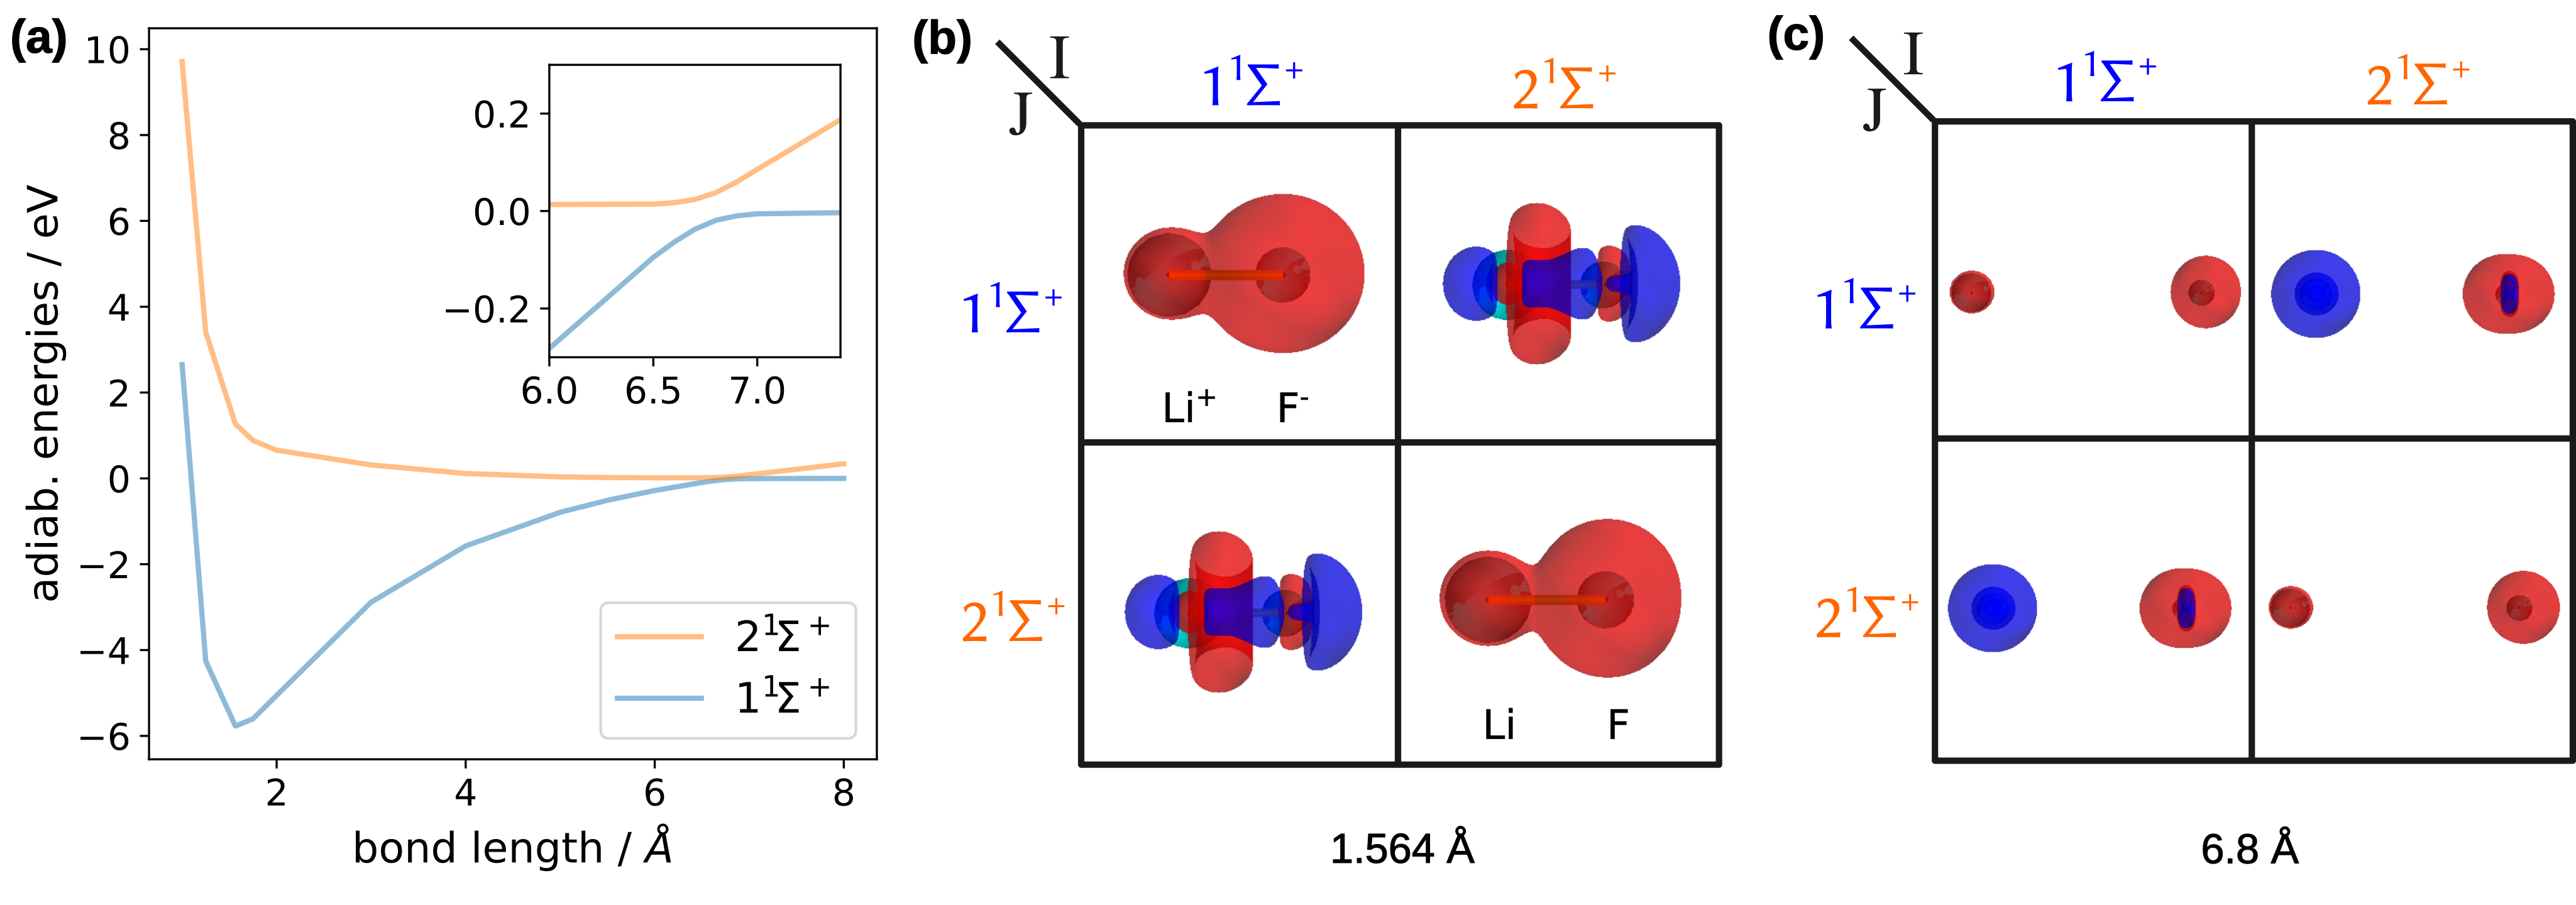
\includegraphics[width=0.9\textwidth]{figures/lithium-fluoride_potential_energies_and_matrix_density.png}
\caption{
\textbf{Lithium-fluoride.}
(a) SA-2-CASSCF(6,21)/aug-cc-pVQZ potential energy curves
for the lowest 2 singlet states with $\Sigma^+$ symmetry, inset: zoom around avoided crossing.
(b,c) Visual representation of the matrix density $D_{IJ}(\vec{r}) = D^{\alpha}_{IJ}(\vec{r}) + D^{\beta}_{IJ}(\vec{r})$
of lithium-fluoride at the experimental bond length of $1.564~\AA$ (b) and at the avoided curve crossing (c).
Diagonal blocks show the electronic state densities for the states $1^1\Sigma^+$ and $2^1\Sigma^+$,
off-diagonal blocks the transition density.
Isovalues of 0.025 and $\approx 0.001$ were used for the state densities and the transition densities, respectively.}
\label{fig:lithium-fluoride_potential_energies_and_matrix_density}
\end{figure}

\begin{figure}[h!]
  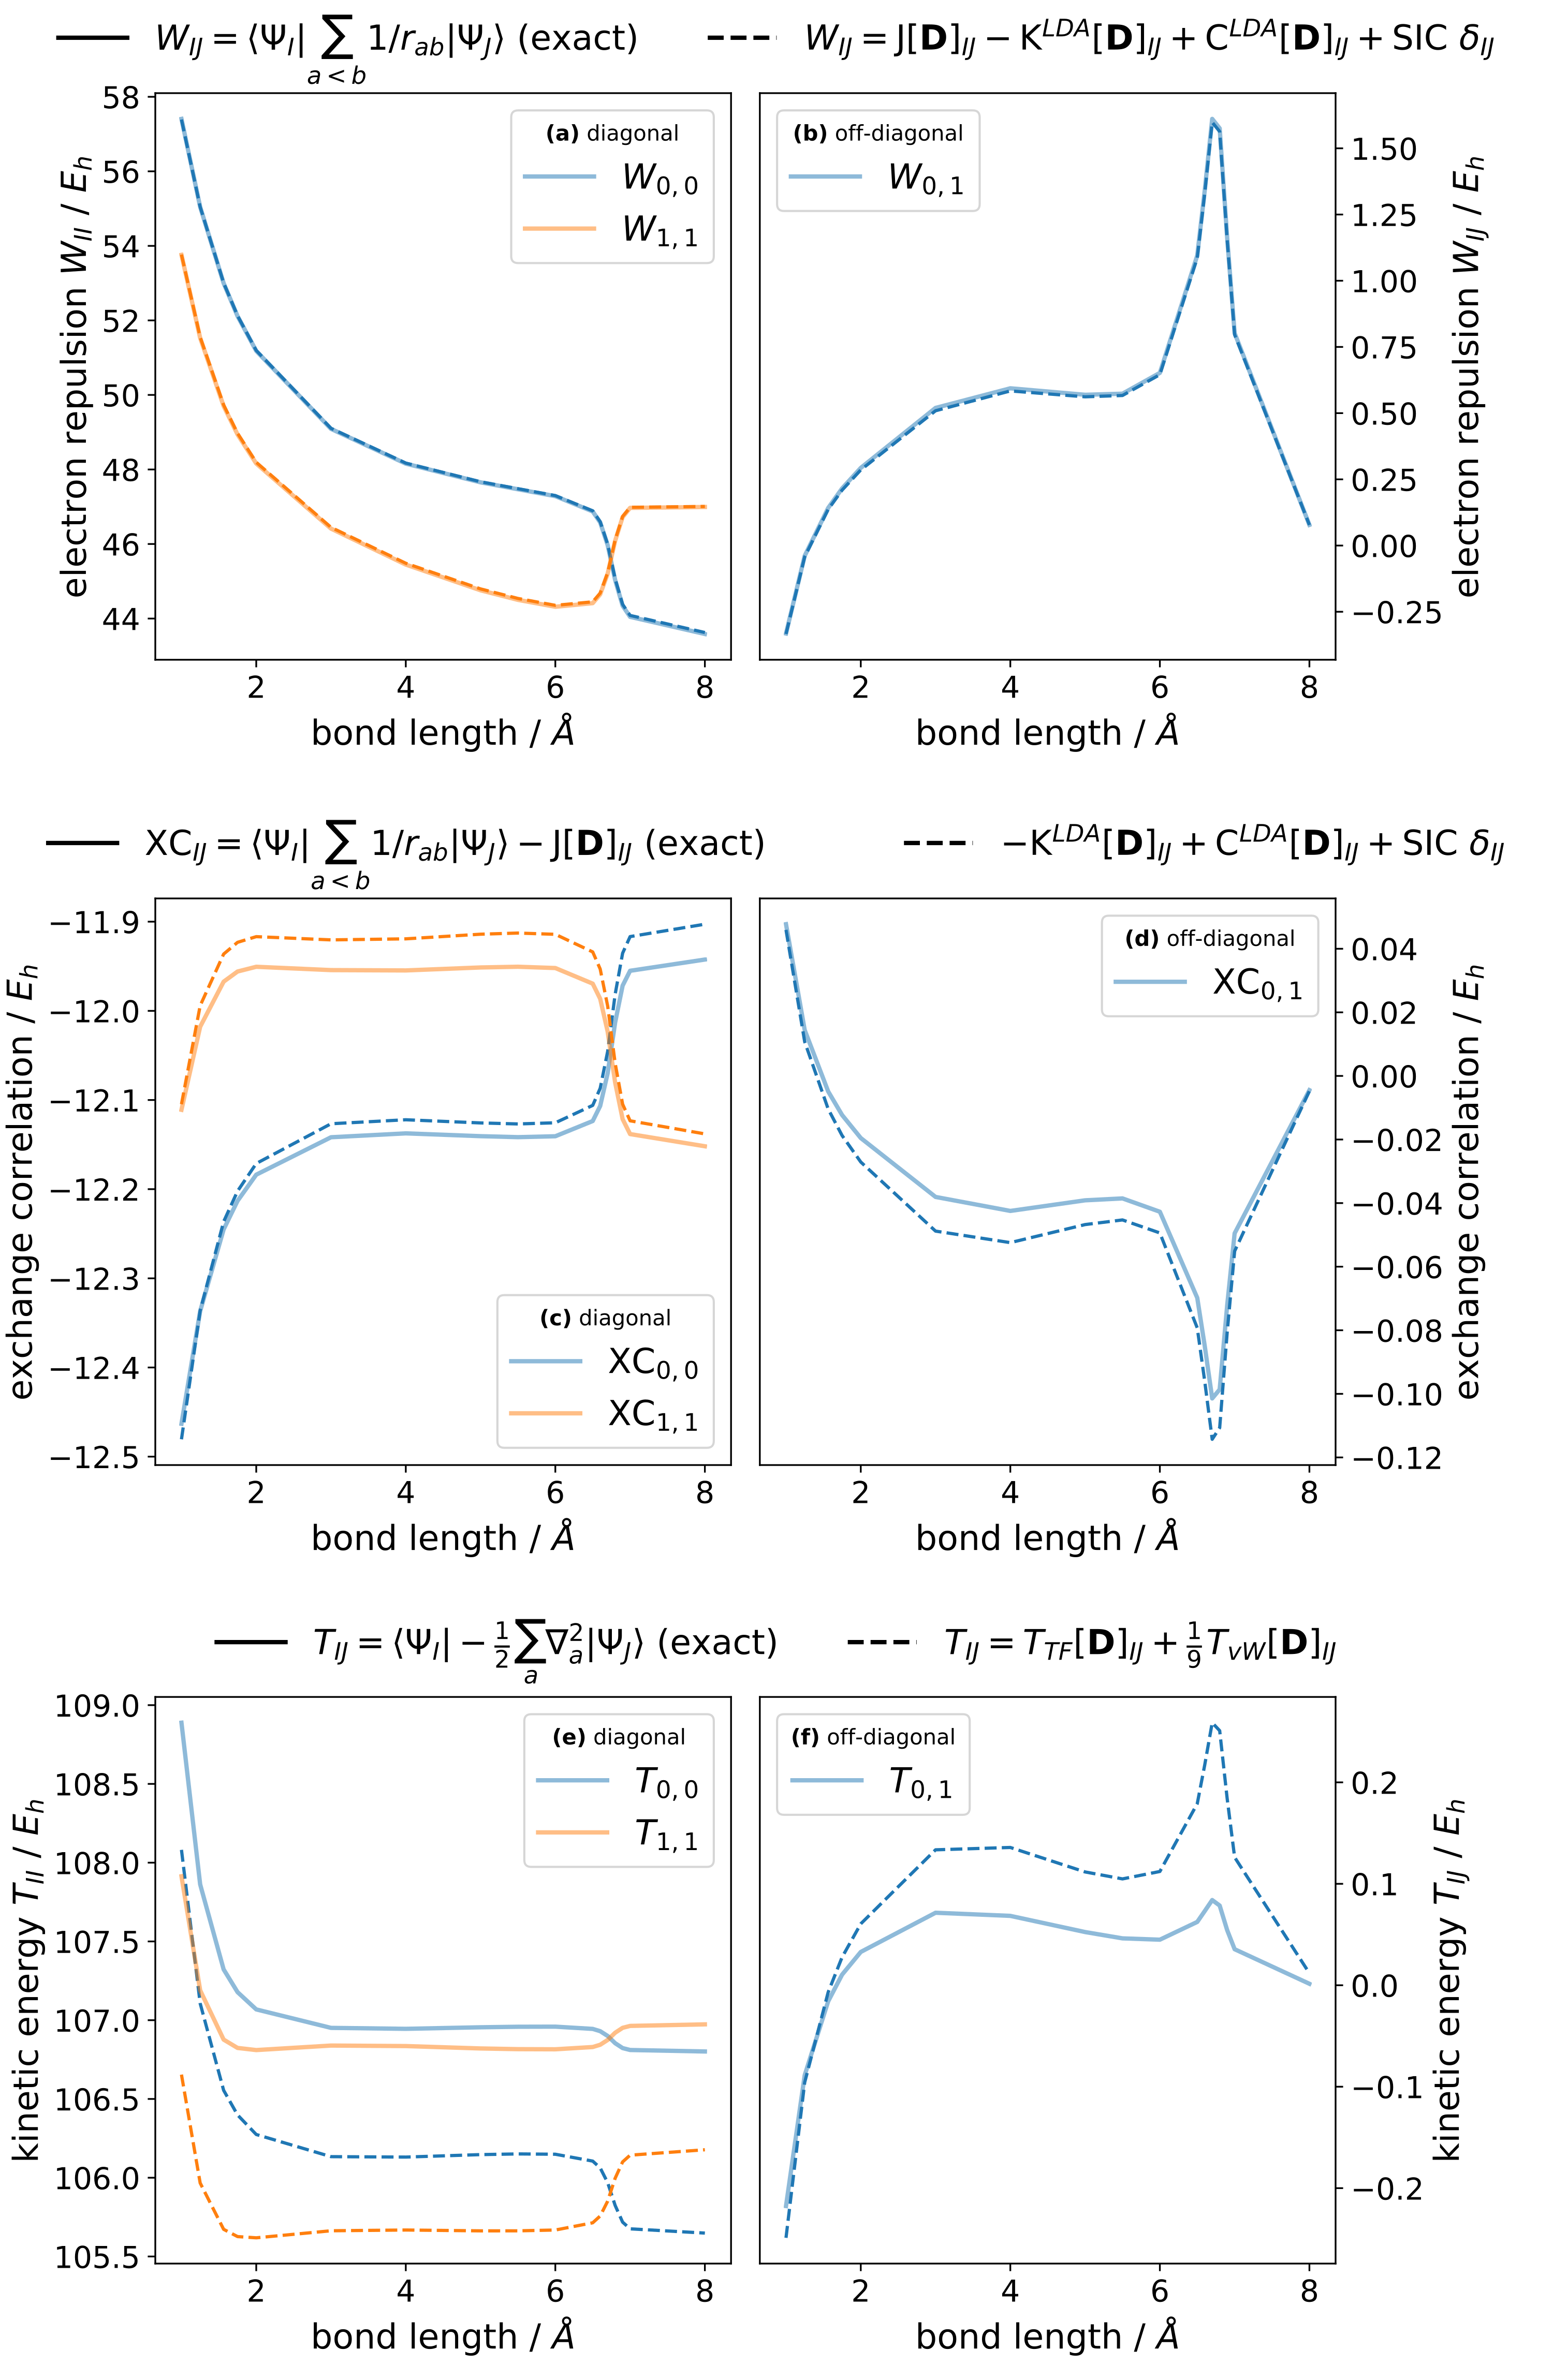
\includegraphics[width=0.8\textwidth]{figures/lithium-fluoride_electron_repulsion_and_kinetic_energies-lda.png}
\caption{
\textbf{Lithium-fluoride.}
Comparison between exact WFT (solid lines) and approximate MSDFT matrix elements (dashed lines)
of the total electron-electron repulsion (a,b), the exchange-correlation (c,d) and the kinetic energy (e,f)
in the basis of the adiabatic eigenstates $1^1\Sigma^+$ ($I=0$) and $2^1\Sigma^+$ ($I=1$).
Left column: diagonal elements, Right column: off-diagonal element.
}
\label{fig:lithium-fluoride_electron_repulsion_and_kinetic_energies}
\end{figure}


%%%%%%%%%%%%%%%%%%%%%% AUTO-GENERATE LATEX CODE (format_latex_table.py) %%%%%%%%%%%%%%%%%%%%%%%%%%%%%%%%%%%%%%%
\sisetup{
round-mode = places,
round-precision = 4,
scientific-notation = fixed,
fixed-exponent = 0,
zero-decimal-to-integer
}

\begin{table}[ht]
  \centering
  \caption{
\normalfont
Electron repulsion and kinetic energy matrices in the basis of the exact eigenstates
$1^1\Sigma^+$ (I=0) and $2^1\Sigma^+$ (I=1) of LiF at the avoided crossing ($6.8~\AA$).
(a) Exact electron repulsion matrix $W_{IJ}^{\text{exact}}$, multistate DFT approximation
{$W[\m{D}]_{IJ} = J[\m{D}]_{IJ} -K^{LDA}[\m{D}]_{IJ} + C^{LDA}[\m{D}]_{IJ} + \text{SIC} \delta_{IJ}$},
Hartree ($J[\m{D}]_{IJ}$), exchange ($-K^{LDA}[\m{D}]_{IJ}$) and correlation ($C^{LDA}[\m{D}]_{IJ}$) matrices
and self-interaction correction for core electrons ($\text{SIC} \delta_{IJ}$).
(b) Exact kinetic energy matrix $T_{IJ}^{\text{exact}}$ and multistate DFT approximation
{$T[\m{D}]_{IJ} = T_{\text{TF}}[\m{D}]_{IJ} + \frac{1}{9} T_{\text{vW}}[\m{D}]_{IJ}$},
Thomas-Fermi ($T_{\text{TF}}[\m{D}]_{IJ}$) and von-Weizs\"{a}cker ($T_{\text{vW}}[\m{D}]_{IJ}$)
kinetic energy matrices.
All energies are in Hartree.}
\label{tbl:lithium_fluoride_electron_repulsion_and_kinetic}

  \medskip

  \begin{tabular}{SSSS}
    \toprule
    \multicolumn{4}{c}{{\textbf{(a)} electron repulsion, matrix elements ($I$,$J$)}} \\
        & {(0,0)} & {(1,1)} & {(0,1)} \\
    \midrule
    {$W_{IJ}^{\text{exact}}$} & 45.033933 & 46.086460 & 1.575356 \\
    {$W[\m{D}]_{IJ}$} & 45.065477 & 46.108180 & 1.563310 \\

    \midrule
    {$J[\m{D}]_{IJ}$} & 57.046943 & 58.166887 & 1.673967 \\
    {$-K^{LDA}[\m{D}]_{IJ}$} & -10.612500 & -10.683227 & -0.101446 \\
    {$C^{LDA}[\m{D}]_{IJ}$} & -0.792414 & -0.798927 & -0.009211 \\
    {$\text{SIC} \delta_{IJ}$} & -0.576553 & -0.576553 & -0.000000 \\

    \bottomrule
  \end{tabular}

  \bigskip

  \begin{tabular}{SSSS}
    \toprule
    \multicolumn{4}{c}{{\textbf{(b)} kinetic energy, matrix elements ($I$,$J$)}} \\
        & {(0,0)} & {(1,1)} & {(0,1)} \\
    \midrule
    {$T_{IJ}^{\text{exact}}$} & 106.854077 & 106.920529 & 0.078547 \\
    {$T[\m{D}]_{IJ}$} & 105.824213 & 105.996851 & 0.250928 \\

    \midrule
    {$T_{\text{TF}}[\m{D}]_{IJ}$} & 96.884252 & 97.082948 & 0.282858 \\
    {$T_{\text{vW}}[\m{D}]_{IJ}$} & 80.459645 & 80.225123 & -0.287369 \\

    \bottomrule
  \end{tabular}
\end{table}
%%%%%%%%%%%%%%%%%%%%%% END OF AUTO-GENERATE LATEX CODE %%%%%%%%%%%%%%%%%%%%%%%%%%%%%%%%%%%%%%%%%%



\FloatBarrier

\section{Conclusion}
\label{sec:conclusion}

The effective Hamiltonian in the subspace of the lowest electronic states is an analytic matrix functional
of the matrix density and does not depend on the number of electronic states.
In contrast to the $\Delta$SCF method, where a ground state functional is applied to the density of a single excited state configuration,
the multistate functional yields both the energies of the configurations and the interactions between them.
By construction the average energy of the lowest states is invariant under basis transformations within the subspace.
When turning ground state functionals into multistate functionals, ambiguities arise because scalar descriptors of the
density become non-commuting matrices. As illustrated for the kinetic energy, exact conditions of the unknown functional
can help to constrain its functional form.

A simple LDA-like multistate functional was tested on the dissociation curve of LiF.
Both diagonal and off-diagonal matrix elements of the electron-electron repulsion operator are reproduced well
when the exact matrix density is used as input.
The exchange-correlation part of the state interaction is dominated by the exchange term,
while correlation is an order of magnitude smaller.
The tested functional is not yet suitable for reliable calculations,
but mostly so because the errors of the diagonal kinetic energy are so huge,
while the errors of the off-diagonal elements are acceptable.

A limitation of this work is that the matrix density was not determined by minimizing the subspace energy.
Using an efficient parameterization of the matrix density \cite[theorem (3)]{Lu2022JPCL} \cite{Lu2022fundamental},
multi-configurational self-consistent field calculations with an effective Hamiltonian computed from the multistate functional
should be possible. This is left for future work.

If a good approximation to the universal mulitstate functional
were known and it were somehow possible to restrict the minimization to valid Fermionic matrix densities,
the multistate DFT of Lu and Gao would open the way for studying neutral excitations in very large systems
in the spirit of orbital-free DFT.

%, but first better matrix functionals of GGA quality are needed.



% Need more exact conditions (such as for vW functional, exact 1e )

%A limitation of this work is that the parameterization of the matrix density in terms of no more than $N^2$ ($N$ = number of states)
%non-orthogonal Slater determinants built from $n \times N^2$ orbitals ($n$ = number of electrons)
%suggested in theorem (3) of Ref.~ \cite{Lu2022JPCL} (and explored further in Ref.~\cite{Lu2022fundamental}) has not been implemented yet.
%So with the current computer program it was
%not possible to find the matrix density that minimizes the multistate energy. This is left for future work, if the method
%should turn out to be promising.

% Correlation energy seems to go the wrong way.

% Diagonal elements are trivial. One could have just applied a ground state functional to the density that belongs to a configuration
% which is orthogonal to the ground state, as done in Delta-SCF. But the off-diagonals are new.... (something like that)

%The resulting functional $\mathcal{F}$ is not suitable for reliable calculations,
%but mostly so because the errors of the diagonal kinetic
%energy are so huge,
%while the errors of the off-diagonal elements are perfectly acceptable.

%Nevertheless this study provides a clean picture of how well matrix functionals derived from simple ground state functionals
%like LDA can approximate the off-diagonal elements of the Hamiltonian matrix using only the matrix density as input.
% Searching for better matrix functionals is therefore worth the effort.


%%%%%%%%%%%%%%%%%%%%%%%%%%%%%%%%%%%%%%%%%%%%%%%%%%%%%%%%%%%%%%%%%%%%%
%% The "Acknowledgement" section can be given in all manuscript
%% classes.  This should be given within the "acknowledgement"
%% environment, which will make the correct section or running title.
%%%%%%%%%%%%%%%%%%%%%%%%%%%%%%%%%%%%%%%%%%%%%%%%%%%%%%%%%%%%%%%%%%%%%
\begin{acknowledgement}
%A.H. thanks Prof. T. Suzuki for the kind support.
There is no funding to declare.
\end{acknowledgement}


%%%%%%%%%%%%%%%%%%%%%%%%%%%%%%%%%%%%%%%%%%%%%%%%%%%%%%%%%%%%%%%%%%%%%
%% The same is true for Supporting Information, which should use the
%% suppinfo environment.
%%%%%%%%%%%%%%%%%%%%%%%%%%%%%%%%%%%%%%%%%%%%%%%%%%%%%%%%%%%%%%%%%%%%%
\begin{suppinfo}
Comparison of paramagnetic and ferromagnetic correlation energy,
proof of Klein's trace inequality,
proof of Lieb-Oxford bound for Coulomb energy of subspace.

\textbf{Code and Data Availability:}
All calculations can be repeated on a desktop computer using the python scripts
in the github repository
\url{https://github.com/humeniuka/multistate_density_functionals-v1/}.
The program package and data are archived at \url{https://zenodo.org/TODO_ADD_URL}.

\end{suppinfo}

%%%%%%%%%%%%%%%%%%%%%%%%%%%%%%%%%%%%%%%%%%%%%%%%%%%%%%%%%%%%%%%%%%%%%
%% The appropriate \bibliography command should be placed here.
%% Notice that the class file automatically sets \bibliographystyle
%% and also names the section correctly.
%%%%%%%%%%%%%%%%%%%%%%%%%%%%%%%%%%%%%%%%%%%%%%%%%%%%%%%%%%%%%%%%%%%%%
\bibliography{references}

\end{document}
